\documentclass[anonymous,timestamp,review,acmtog]{acmart}

\usepackage{booktabs} % For formal tables
%\usepackage{subfigure}
\usepackage{subcaption}
\usepackage{graphicx}
%\graphicspath{{C:/Users/black/OneDrive/Documents/UT/Research/Shell/MoistInducedSim}}

\newcommand{\ba}{\mathbf{a}}
\newcommand{\bb}{\mathbf{b}}
\newcommand{\bc}{\mathbf{c}}
\newcommand{\bg}{\mathbf{g}}
\newcommand{\br}{\mathbf{r}}
\newcommand{\bff}{\mathbf{f}}
\newcommand{\bv}{\mathbf{v}}
\newcommand{\be}{\mathbf{e}}
\newcommand{\bd}{\mathbf{d}}
\newcommand{\bF}{\mathbf{F}}
\newcommand{\bJ}{\mathbf{J}}
\newcommand{\bx}{\mathbf{x}}
\DeclareMathOperator{\tr}{tr}
\newcommand{\hn}{\hat{\mathbf{n}}}
\newcommand{\fT}{\mathcal{T}}

\acmPrice{15.00}

% The next six lines come directly from the completed rights form.
% You MUST replace them with the lines specific to your accepted work.
\copyrightyear{2018}
\acmYear{2018}
\setcopyright{rightsretained}
\acmConference{Conference Name}{Conference Date and Year}{Conference Location}
\acmDOI{10.1145/8888888.7777777}
\acmISBN{978-1-4503-1234-5/17/07}

% Use the "authoryear" citation style, and make sure citations are in [square brackets].
\citestyle{acmauthoryear}
\setcitestyle{square}

% A useful command for controlling the number of authors per row.
% The default value of "authorsperrow" is 2.
\settopmatter{authorsperrow=2}

% end of preamble.

\begin{document}

% Title. 
% If your title is long, consider \title[short title]{full title} - "short title" will be used for running heads.
\title{Physical Simulation of Moisture Induced Thin Shell Deformation}

% Authors.
\author{Hsiao-yu Chen}
\affiliation{%
  \institution{University of Texas at Austin}}

\author{Etienne Vouga}
\affiliation{%
  \institution{University of Texas at Austin}}

% This command defines the author string for running heads.
%\renewcommand{\shortauthors}{DeJohnette, Rowland-Smith, Badeeri, and Foyt}

% abstract
\begin{abstract}

\end{abstract}

%CCS
\begin{CCSXML}
%<ccs2012>
%<concept>
%<concept_id>10010147.10010371.10010372</concept_id>
%<concept_desc>Computing methodologies~Rendering</concept_desc>
%<concept_significance>500</concept_significance>
%</concept>
%<concept>
%<concept_id>10010147.10010371.10010372.10010374</concept_id>
%<concept_desc>Computing methodologies~Ray tracing</concept_desc>
%<concept_significance>500</concept_significance>
%</concept>
%</ccs2012>
\end{CCSXML}

%\ccsdesc[500]{Computing methodologies~Rendering}
%\ccsdesc[500]{Computing methodologies~Ray tracing}
%
%%keywords
%\keywords{ray tracing, global illumination, octrees, quadtrees}
%
%% A "teaser" figure, centered below the title and authors and above the body of the work.
%\begin{teaserfigure}
%  \centering
%  \includegraphics[width=6.0in]{aaafiles/fountain}
%  \caption{Drumheller Fountain, The University of Washington, Seattle WA.}
%\end{teaserfigure}
%
%% Processes all of the front-end information and starts the body of the work.
\maketitle

\section{Introduction}


\paragraph{Contribution} We present a low-order discrete shell model tailored to simulating non-uniform, anisotropic, differential swelling and shrinking of thin shells. In contrast to previous methods for simulating related phenomena, such as burning and growth, our formulation builds on discrete geometric shell theory and supports arbitrary rest curvature and strain, and physical settings such as thickness and Lam\'{e} parameters. We couple our shell model to a simple formulation of moisture diffusion in both the lateral and thickness directions, which takes into account anisotropy of the material grain. In a series of experiments, we show that our model successfully predicts the qualitative behavior of thin shells undergoing complex, dynamic deformations due to swelling or shrinking, such as occurs when paper is moistened, leaves dry in the sun, or thin plastic melts.

\subsection{Related Work}
\paragraph{Simulating Burning/Melting/Swelling} Several papers look at related problems, such as evolving the boundary of a burning or melting solid, without incorporating curling/wrinkling and other elastic deformations of the solid. Melek and Keyser~\shortcite{Melek2003,Melek2005} simulate pyrolysis and heat diffusion of burning objects, but do not consider elastic deformation of the burning objects. Losasso et al~\shortcite{Losasso2006} proposed tracking of the burning boundary of thin shells using an adaptive level set on the shell. Some of the deformation can be qualitatively approximated by mapping physical quntities like heat and moisture to cells of a coarse grid around the object, deforming the cage, and mapping the deformation back onto the shell (as in Free Form Deformation); this approach was proposed by Melek and Keyser~\shortcite{Melek2007} and adopted by Liu et al~\shortcite{Liu2009}. Most similar to our work is the method of Jeong et al~\shortcite{Jeong2011,Jeong2013}, which uses a \emph{bilayer} of springs (a triangle mesh and its circumcentric dual, offset a distance from the primal mesh) to represent the shell. The bilayer allows the method to capture \emph{differential} growth due to gradients in moisture concentration across the thickness of leaves, leading to visually impressive simulations of leaves curling as they dry. Our work is based on the same fundamental idea (representing the shell using rest geometry that varies linearly through the thickness) but couched in the machinery of differential geometry; our formulation allows us to easily incorporate non-zero rest curvature, machine direction, and a physical material model.

Steps towards a principled physical model include the use of a mass-spring network to represent the shell, with update rules for how spring rest lengths should change due to physical processes in the shell. Such rules are simplest to formulate in the case where growth or shrinkage is uniform through the shell thickness, and the shell can be represented using a single spring layer; Larboulette et al~\shortcite{Larboulette2013} present such a rule, which includes handling of the \emph{machine direction} of paper: a bias in the orientation of the fibers composing the paper which causes the paper to swell anisotropically. We adopt this parameter in our material model. 

\paragraph{Mechanics of Shells}
The mathematics and geometry underpinning the physics of thin shells is a venerable topic: Ciarlet's book~\shortcite{Ciarlet2000} on elasticity as applied to shells offers a thorough overview. Our work is based on the common \emph{Kirchhoff-Love} assumption that the shell does not undergo any transverse shear; i.e., that the shell volume is foliated by normal offsets of the shell's \emph{midsurface}: the problem of studying deformation of the 3D shell volume then reduces to that of deformation of a 2D surface, and tools from Riemannian geometry can be applied~\cite{Simo1989}. (We adopt the so-called ``intrinsic'' view~\cite{Neff2004} that shells can be understood in terms of Kirchhoff-Love and geometric principles, as this view allows us to easily discretize shell physics by leveraging discrete differential geometry, but we note in passing that the validity of the Kirchhoff-Love assumption, and of reduced shell models in general, remains unsettled, and the literature documents numerous alternative shell theories.) One key property of the shells we want to simulate is that they are \emph{non-Euclidean}: they do not have a rest (strain-free) state that is realizable in three-dimensional space. Non-Euclidean shells have received substantial attention recently in the physics community~\cite{Klein2007,Kim2012}, thanks to their potential applications in fabrication and robotics, and their connection to biological growth; Sharon and Efrati~\cite{Efrati2009,Sharon2010} pioneered the study of shell mechanics in this setting.

For the sake of being self-contained, we briefly review the geometric foundations of shell mechanics in Section \ref{sec:continuous}.

\paragraph{Computational Modeling of Thin Shells} 
Thin shells first caught the interest of the graphics community in the context of simulating cloth~\cite{Baraff1998,Bridson2002}. These early methods tended to focus on thin \emph{plates}, i.e. shells that are rest flat, and formulate shell dynamics either in terms of either hinge-based bending energies~\cite{Sullivan2008,Tamstorf2013} or the insight that the bending energy can be written in terms of the intrinsic Laplace-Beltrami operator applied to the shell's embedding function~\cite{Bobenko2005,Bergou2006,Wardetzky2007}. Grinspun et al~\shortcite{Grinspun2003} introduced to graphics the simulation of shells with non-flat rest curvature. Their formulation is based on \emph{differences of squared mean curvature}, leading to a simple and easy-to-discrete bending energy; this model is physically suspect, however: consider a half-cylinder at rest when curled around the $x$-axis. Unbend the shell and re-bend it around the $y$-axis; the deformed configuraiton's strain cannot be captured by looking at mean curvature alone, as it is pointwise identical to the mean curvature of the rest configuration. Complete support for rest curvature requires a bending energy that incorporates full information about the extrinsic deformation of the shell~\cite{Grinspun2006}. One recent such discrete energy is described in Weischedel's under-appreciated work on discrete Cosserat shells~\shortcite{Weischedel2012}; our exposition is modeled closesly on hers, though we make different modeling choices (we use an intrinsic rather than Cosserat shell model, and require more flexible handling of the shell rest geometry).

Higher-order methods for simulating shells (including with e.g. NURBS or subdivision elements) are common in computational mechanics and isogeometric analysis~\cite{Batoz1980,Bathe1983,Cirak2000,Kiendl2009,Benson2010,Bandara2018} and have also been proposed for computer graphics~\cite{Wawrzinek2011}. High-order methods have some obvious advantages (better convergence behavior in the thin limit, especially for shell deformations involving large strains; continuous surface normals) at the cost of additional computational cost and complexity, especially when handling contact.

In this paper, we ignore the problem of mesh tessellation, or of adapting the mesh in response to either large deflections or large amounts of growth; such remeshing is an important component of a practical shell simulation but orthogonal to our focus on shell dynamics. ArcSim~\cite{Narain2012} incorporates a method of adaptive remeshing while avoiding significant popping artifacts, and has been used to generate impressive simulations of creasing paper. Vetter et al~\shortcite{Vetter13} study the companion problem of remeshing due to large in-plane growth, and present a solution based on adaptive Loop subdivision.

\section{Continuous Formulation} \label{sec:continuous}
Before describing our discretization of shells, we briefly review the formulation in the continuous setting, as this formulation will guide our discretization. 

\paragraph{Shell Geometry} We can represent shells $S\subset \mathbb{R}^3$ of thickness $h$ by a parameter domain $\Omega$ in the plane and an embedding $\phi: \Omega\times [-h/2, h/2]\to\mathbb{R}^3$ with $S$ the image of $\phi$ (see Figure~\ref{fig:XXX}). We adopt the common \emph{Kirchhoff-Love} assumption that the shell does not undergo any transverse shear; i.e., that the shell volume is foliated by normal offsets of the shell's \emph{midsurface} $\br:\Omega\to\mathbb{R}^3$. In other words,
$$\phi(x,y,z) = \br(x,y) + z\hn(x,y)$$
where $\hn = (\br_x \times \br_y)/\|\br_x \times \br_y\|$ is the midsurface normal. The shell's deformation is thus completely determined by the deformation of the midsurface. The metric $\bg$ on the slab $\Omega \times [-h/2,h/2]$, pulled back from $\mathbb{R}^3$, can be expressed in terms of the geometry of the midsurface:
\begin{equation}
\bg = \left[\begin{array}{cc}\ba - 2z\bb + z^2 \bc & 0\\0 & 1\end{array}\right],\label{eq:offset}
\end{equation}
where
$$\ba = d\br^Td\br \quad \bb = -d\br^Td\hn \quad \bc = d\hn^Td\hn$$
are the classical first, second, and third fundamental forms of the surface $\br$.

Oftentimes, the parameterization domain of a thin shell is assumed to be also the rest state of the shell, so that the strain in the material of the shell can be determined directly from looking at $\bg$. We cannot assume this: consider for instance a piece of paper whose center has been moistened by spilled coffee. The fibers in the coffee stain stretch; since they are confined by the surrounding non-wet region of the paper, the paper cannot globally stretch in such a way that both the wet and dry regions of the paper are simultaneously at rest. Instead, the paper will \emph{buckle} out of plane, into a shape that compromises between relaxing the in-plane (stretching) strain and the introduced bending strain. At this point the paper's rest state is \emph{non-Euclidean}---it is impossible to find any embedding of the paper into $\mathbb{R}^3$ that is entirely strain-free.

We therefore record the rest state of the shell using a \emph{rest metric} $\bar\bg(x,y,z).$\footnote{Here and throughout the paper, we use an overbar to denote quantities associated to the shell rest state.} Since our model is tailored to simulating differential in-plane swelling or shrinking across the thickness of the shell, we make the simplifying assumption that this rest metric is linear in the thickness direction, and does not affect the shell thickness:
$$\bar\bg(x,y,z) = \bar\ba(x,y) - 2z\bar\bb(x,y).$$
A shell that begins a simulation at rest will simply have $\bar\ba = \ba$ and $\bar\bb = \bb$; similarly, in the case that the shell \emph{does} have a rest state $\bar\br$ that is isometrically embeddable in $\mathbb{R}^3$, $\ba$ and $\bb$ are the first and second fundamental forms of the surface $\bar\br$. Therefore $\ba$ and $\bb$ can be thought of as representing the ``rest metric'' and ``rest curvature'' of the shell, respectively.\footnote{We stress, though, that these labels are to provide intuition only---$\bar\ba$ and $\bar\bb$ must not, and generally will not, satisfy usual relationships from differential geometry such as the Gauss-Codazzi-Mainardi equations.}

Finally, we cannot assume that the shell has uniform density, since different parts of the shell might gain or lose mass due to absorbing or releasing moisture. We therefore allow the density per unit \emph{rest} volume $\rho(x,y)$ to vary over $\Omega$. (In principle, we could also model the variation in density across the shell thickness; however doing so leads only to a small ($O(h^3)$) correction to the shell's kinetic energy, and since the swelling phenomena we are interested in simulating tend to happen over relatively long time scales, there is no need for such accuracy.)

To summarize, our parameterization of thin shells involves the following kinematic elements:
\begin{itemize}
\item a thickness $h$ and parameterization domain $\Omega\subset\mathbb{R}^2$, both of which are fixed over the course of the simulation;
\item an embedding $\br:\Omega\to\mathbb{R}^3$ representing the shell midsurface's ``current''/``deformed'' geometry, and which evolves over time. From this midsurface embedding, the embedding of the full shell volume $\phi$, and the midsurface fundamental forms, can be calculated;
\item a rest metric and density, parameterized by the pair of tensor field $\bar\ba, \bar\bb$ and a scalar field $\rho$ over $\Omega$, respectively. These might also evolve over time, due to changes in the shell rest state via growth or shrinkage.
\end{itemize}

\subsection{Shell Dynamics}
Motivated by the common observation that a sufficiently thin shell bends much more readily than it will stretch, we assume that the shell's deformation involves \emph{large rotations} but only small in-plane strain of the midsurface: $\|\bar\ba^{-1}\ba-I\|_{\infty} < h.$ We also assume that the shell's material is uniform and isotropic. The simplest constitutive law consistent with these assumptions is to use a St. Venant-Kirchhoff material model\footnote{The neo-Hookean material model is also popular in computer graphics and could be used instead, although there is little benefit to doing so when simulating thin shells since strains are typically small.} together with Green strain; it can be shown~\cite{XXX} that these choices yield an elastic energy  density~(the \emph{Koiter shell model}) that can be approximated up to $O(h^4)$ by
\begin{equation}
W(x,y) = \left(\frac{h}{4} \|\bar\ba^{-1}\ba - I\|^2_{SV} + \frac{h^3}{12}\|\bar\ba^{-1}(\bb-\bar\bb)\|^2_{SV}\right)\sqrt{\det \bar\ba} \label{eq:koiter}
\end{equation}
where $\|\|_{SV}$ is the ``St. Venant-Kirchhoff norm''\cite{Weischedel2012}
$$\|M\|_{SV} = \frac{\alpha}{2}\tr^2 M + \beta \tr\left(M^2\right),$$
for Lam\'e parameters $\alpha, \beta$. In terms of the Young's modulus $E$ and Poisson's ratio $\nu$,
$$\alpha = \frac{E\nu}{(1+\nu)(1-2\nu)}, \quad \beta = \frac{E}{2(1+\nu)}.$$

We thus have a formulation of kinetic energy and potential energy
$$T[\dot\br] = \int_{\Omega} h\rho\|\dot\br\|^2 \sqrt{\det\bar\ba}\,dxdy, \quad V[\br] = \int_{\Omega} W(x,y)\,dxdy,$$
to which additional external energies and forces (gravity, constraint forces, etc) can be added to yield equations of motion via the usual principle of least action.

\section{Discretization}
We approximate the midsurface $\br$ with a triangle mesh $(V,E,F)$; the positions of the vertices $\bv = [\bv_1, \bv_2\,\ldots]$ take the place of the embedding function $\br$. The general strategy we will use is to assume that $\ba$ and $\bb$, as well as their rest counterparts $\bar\ba$ and $\bar\bb$, are constant over each face of a triangle mesh representing the shell midsurface; it will then be relatively straightforward to write down a discrete analogue of the Koiter elastic energy density in Equation~\eqref{eq:koiter}. 

\paragraph{Discrete Shell Model} As in the continuous setting, the discrete shell does not necessarily have a rest state embeddable as a mesh in $\mathbb{R}^3$, making it impossible to parameterize the deformed configuration of the shell in terms of the rest configuration; additionally we do not want to assume (or compute) a global parameterization of the midsurface. Instead, we independently parameterize each triangle in its own barycentric coordinates (see Figure~\ref{XXX}). Let $\bff_{ijk}$ be a face in $F$ containing the vertices $\bv_i$,$\bv_j$, $\bv_k$, and denote by $\fT$ the canonical unit triangle with vertices $(0,0)$, $(1,0)$, $(0,1)$. Then locally the face $\bff_{ijk}$ is embedded by the affine function
$$\br_{ijk}:\fT\to\mathbb{R}^3, \quad \br_{ijk}(u_1,u_2) = \bv_i + u_1(\bv_j-\bv_i)+u_2(\bv_k-\bv_i);$$
under this embedding, the Euclidean metric on face $\bff_{ijk}$ pulls back to the constant first fundamental form
$$\ba_{ijk} = \left[\begin{array}{cc} \|\bv_j-\bv_i\|^2 & (\bv_j-\bv_i)\cdot(\bv_k-\bv_i)\\
(\bv_j-\bv_i)\cdot(\bv_k-\bv_i) & \|\bv_k-\bv_i\|^2\end{array}\right]$$
on $\fT$. If we are given an explicit rest configuration $\bar\bv_i$ of the shell, we can compute the rest first fundamental form $\bar\ba_{ijk}$ analogously; or alternatively we can set $\bar\ba_{ijk}$ to any desired symmetric positive-definite $2\times 2$ matrix. Notice that any such matrix corresponds to some choice of ``rest lengths'' for the edges of face $\bff_{ijk}$ that obey the triangle inequality, but that two faces sharing a common edge do not necessarily agree about that length. 

These discrete fundamental forms are enough to discretize the stretching term in Equation~\eqref{eq:koiter}: each face contributes a term 
\begin{align*}
&\int_{\fT} \frac{h}{4} \|\bar\ba_{ijk}^{-1}\ba_{ijk} - I\|^2_{SV}\sqrt{\det{\bar\ba_{ijk}}}\\
&\quad = \frac{h}{8} \|\bar\ba_{ijk}^{-1}\ba_{ijk} - I\|^2_{SV}\sqrt{\det{\bar\ba_{ijk}}}.
\end{align*}
This energy is quartic in the positions of the mesh vertices, and is exactly the energy of constant-strain triangle stretching elements commonly used in cloth simulation.

For the bending term, we also need a discretization of the second fundamental form. Here there is a significant departure between the smooth theory and the discrete approximation: we would like to apply the Kirchhoff=Love principle to extrude the mid-surface into a shell volume, but unfortunately distance offsets of triangle meshes are no longer guaranteed to be triangle meshes (or even piecewise-affine). One can instead look at weaker notions of mesh parallellity~\cite{Bobenko2010}:
\begin{itemize}
\item \emph{vertex offsets} require choosing a normal at each mesh vertex (itself a problem without an obvious solution), and moving each vertex a constant distance along this normal usually does not result in faces parallel to the original faces;
\item \emph{edge offsets} likewise do not guarantee parallel faces;
\item \emph{face offsets} are not conforming: moving each face around a vertex of valence four or higher in their normal direction yields new faces that are not guaranteed to still intersect at a common point.
\end{itemize}

We use the discretization that arises from edge parallelity, leading to the so-called ``mid-edge'' discretization of the second fundamental form~\cite{Grinspun2006,Weischedel2012}: let $\be_i$ denote the edge opposite vertex $i$ on face $\bf_{ijk}$, and define the \emph{mid-edge normal} $\hn_i$ by:
\begin{itemize}
\item the face normal $\frac{(\bv_j-\bv_i)\times (\bv_k-\bv_i)}{\|(\bv_j-\bv_i)\times (\bv_k-\bv_i)\|}$, if $\be_i$ is a boundary edge;
\item the mean of the face normals of the two faces incident on $\be_i$, otherwise.
\end{itemize}

Let $\bff_{ijk}^{\epsilon}$ denote the triangle formed by offsetting all of $\bff_{ijk}$'s edges in their mid-edge normal direction by a distance $\epsilon$, and let $\ba^{\epsilon}_{ijk}$ be the discrete first fundamental form of that offset triangle. Then the discrete second fundamental form $\bb$ can be defined, by analogy to Equation~\eqref{eq:offset}, as the first-order correction
$$\ba^{\epsilon}_{ijk} = \ba_{ijk} - 2\epsilon \bb_{ijk} + O(\epsilon^2),$$
leading to the formula
$$\bb_{ijk} = \frac{1}{2}\left[\begin{array}{cc}(\hn_i-\hn_j)\cdot(\bv_i-\bv_j) & (\hn_i-\hn_j)\cdot(\bv_i-\bv_k) \\ (\hn_i-\hn_k)\cdot(\bv_i-\bv_j) & (\hn_i-\hn_k)\cdot(\bv_i-\bv_k)\end{array}\right].$$
(Alternatively, this formula can be derived by discretizing the relation $\bb = -d\br^Td\hn$ using divided differences). Although it may not appear so at first, the matrix $\bb_{ijk}$ is always symmetric (since each mid-edge normal is orthogonal to that edge); it is not in general positive-definite.\footnote{As observed by Grinspun et al~\shortcite{Grinspun2006}, the \emph{shape operator} $d\hn$ in the continuous setting always maps tangent vectors to tangent vectors, whereas in the discrete setting the finite difference of mid-edge normals is not always parallel to the mesh triangle. This discrepancy is a consequence of the failure of edge-offset meshes to also be face-offsets. Corrections to the shape operator have been proposed to remedy this quirk, though we found them unnecessary (and in any case, any components of $d\hn$ that lie orthogonal to the face are annihilated when forming the second fundamental form $-d\br^Td\hn$).} We represent the rest second fundamental form $\bar\bb_{ijk}$ by an arbitrary symmetric $2\times 2$ matrix assigned to each face.

\paragraph{Choosing Rest Fundamental Forms}
Depending on the mechanism for growth being simulated, there are several choices for how to set and update $\bar\ba$ and $\bar\bb$:
\begin{itemize}
\item \textbf{No Growth}: A classic shell, whose rest state is fixed, simply has $\bar\ba=\ba^0$ and $\bar\bb=\bb^0$, where $\ba^0$ denotes the first fundamental form induced by $\bv^0$, the positions of the midsurface vertices at the beginning of the simulation. (And if the shell is pre-stressed, $\bar\ba, \bar\bb$ can be adjusted appropriately).
\item \textbf{Pullback Forms}: In the case where the shell's initial configuration is flat, it is natural to align it with a region of the $xy$ plane, and prescribe rest fundamental forms on $\operatorname{im} \br$ in Euclidean $x,y$ coordinates. Let $\bar\ba^{xy}$ and $\bar\bb^{xy}$ be such prescribed forms; these can be sampled per triangle $\bff_{i,j,k}$ and pulled back to the triangle's parameterization domain to give
$$\bar\ba = T^T\bar\ba^{xy}(\bc)T, \qquad  T^T\bar\bb^{xy}(\bc)T,$$
where
$$T = \left[\begin{array}{cc}\bv^0_{j} - \bv^0_{i} & \bv^0_{k}-\bv^0_{i}\end{array}\right]$$
maps from vectors in the barycentric coordinates of $\bff_{ijk}$ to Euclidean space, and $\bc = \frac{1}{3}(\bv_i+\bv_j+\bv_k)$ is the face centroid.

\item \textbf{Isotropic Growth}: In many cases growth is isotropic and uniform through the thickness of the shell (for instance, when plastic shrinks in response to heat, or plant tissue grows through cell division). In this case 
$$\bar\ba = e^{2s_{ijk}}\ba^0, \qquad \bar\bb = \bb^0$$
for a conformal factor $s$ encoding the amount of growth (or shrinking, if negative).

\item \textbf{Linear Differential Swelling}: Porous materials like paper swell when moistened, and differences in water concentration through the thickness of a thin shell can induce metric frustration and buckling. This mechanism is responsible for the buckling of paper when wet, and the curling of leaves as they dry. 

We model this swelling mechanism by assuming that the amount of moisture varies linearly in the thickness direction of the shell, and present the percentage of additional moisture present in the material at the top and bottom of the shell by two scalars $m^+_{ijk}, m^-_{ijk}\in \mathbb{R}$. The additional water content induces swelling, which changes the rest geometry; assuming a linear relationship between rest length and moisture concentration~\cite{iggesund1993paperboard}, moisture expansion coefficient $\mu$ of the paper is defined as
$$\mu = \frac{\Delta L}{L \Delta m}$$
where $\Delta L$ is the change of length of the paper. In this paper, we set the initial moisture of the paper as reference moisture to 0 and the initial length as L. The rest metric of the shell at the top and bottom of the thickness is given by
$$\bar\bg^+ = (1 + m^+\mu)^2(\ba^0 - h \bb^0), \qquad \bar\bg^- = (1+m^-\mu)^2(\ba^0 + h \bb^0),$$
Then
\begin{align*}
\bar\ba &= \frac{(1+m^+\mu)^2 + (1+m^-\mu)^2}{2}\ba^0 + h\frac{(1+m^-\mu)^2 - (1+m^+\mu)^2}{2}\bb^0\\
\bar\bb &= \frac{(1+m^-\mu)^2 - (1+m^+\mu)^2}{2h}\ba^0 + \frac{(1+m^+\mu)^2 + (1+m^-\mu)^2}{2}\bb^0.
\end{align*}

\item\textbf{Piecewise Constant Differential Swelling} Instead of a linear moisture gradient through the thickness, in some cases it is more appropriate to model a piecewise constant moisture profile, such as when modeling bilayers with different material properties. For example, XXX et al~\cite{XXX} fabricate exotic pasta geometries by cooking pasta composed of two layers of different porosity. van Reese et al~\cite{XXX} showed that a bilayer of thickness $h$ with piecewise-constant rest metric
$$\bar\bg(z) = \begin{cases}\bar\bg^+, z>0\\ \bar\bg^-, z<0\end{cases}$$
is \emph{energetically equivalent} to a shell with linearly-varying metric
$$\bar\ba = \frac{\bg^+ +\bg^-}{2}, \qquad \bar\bb = \frac{3}{4h}(\bg^--\bg^+);$$
thus the desired piecewise-constant metric taking into account moisture-induced swelling is
$$\bar\bg^+ = (1 + m^+\mu^+)^2\left(\ba^0 - \frac{2}{3}h \bb^0\right), \quad \bar\bg^- = (1+m^-\mu^-)^2\left(\ba^0 + \frac{2}{3}h \bb^0\right),$$
where $\mu^+$ and $\mu^-$ encode the differing moisture-length relationship in the two layers. Converting this piecewise-constant metric back into the equivalent linear metric gives
\begin{align*}
\bar\ba &= \frac{(1+m^+\mu^+)^2 + (1+m^-\mu^-)^2}{2}\ba^0 + h\frac{(1+m^-\mu^-)^2 - (1+m^+\mu^+)^2}{3}\bb^0\\
\bar\bb &= 3\frac{(1+m^-\mu^-)^2 - (1+m^+\mu^+)^2}{4h}\ba^0 + \frac{(1+m^+\mu^+)^2 + (1+m^-\mu^-)^2}{2}\bb^0.
\end{align*}
\item\textbf{Linear Differential Swelling with Machine Direction} In paper, leaves, and other materials composed of microscopic fibers, swelling induced by moisture is \emph{anisotropic}, since fibers swell more in their circumferential than axial direction. We can model this behavior by storing a \emph{machine direction} $\bd_{ijk}$ per triangle face; this direction, a vector in the barycentric coordinates of the triangle, is the direction in which the fibers are aligned. Given this direction, we can compute the intrinsically orthogonal direction $\bd_{ijk}^{\perp}$ (with $\bd_{ijk}^T \ba_{ijk}^0 \bd_{ijk}^{\perp} =0$), and impose different moisture-length constants $\mu$ and $\mu_{\perp}$ in the $\bd$ and $\bd^{\perp}$ directions, respectively. Then the desired rest metrics at the top and bottom of the shell are 
\begin{align*}
\bar\bg^+ &= T^T M^+ T^{-T} (\ba^0 - h \bb^0) T^{-1}M^+T,\\
\bar\bg^- &= T^T M^- T^{-T} (\ba^0 + h \bb^0) T^{-1}M^-T.
\end{align*}
where 
$$T = \left[\begin{array}{cc} \bd & \bd_{\perp}\end{array}\right]^{-1}$$
transforms from the triangle's barycentric coordinates to the $\bd,\bd_{\perp}$ coordinate system, and
$$M^{\pm} = \left[\begin{array}{cc}
(1 + m^{\pm}\mu) & 0\\0 & (1+m^{\pm} \mu_{\perp})\end{array}\right]$$
anisotropically stretches in the machine direction. As in the previous cases, the rest fundamental forms can be computed from these metrics using the formula
$$\bar\ba = \frac{\bar\bg^++\bar\bg^-}{2}, \qquad \bar\bb = \frac{\bar\bg^- - \bar\bg^+}{2h}.$$
\end{itemize}


\paragraph{Elastic Energy} We can now write down the full elastic energy of the shell, in exact analogy to the Koiter energy:
\begin{align*}
E_{\mathrm{elastic}}(\bv) &= \sum_{\bff_{ijk}\in F} \frac{\sqrt{\det \bar\ba_{ijk}}}{2}\Bigg(\frac{h}{4} \|\bar\ba_{ijk}^{-1}\ba_{ijk} - I\|^2_{SV}\\
&\qquad + \frac{h^3}{12}\|\bar\ba_{ijk}^{-1}(\bb_{ijk}-\bar\bb_{ijk})\|^2_{SV}\Bigg)
\end{align*}
It is worth making a few observations about this energy. First, the matrices $\ba$, $\bar\ba$, etc. are \emph{coordinate-dependent}: replacing the parameterization domain $\fT$, or even cyclically permuting the order of vertices around a face, would alter the values in the matrix. However, the generalized eigenvalues of $\ba-\bar\ba$ and $\bb-\bar\bb$ with respect to the inner product $\bar\ba$ are coordinate-\emph{independent}, as is the total energy. Perhaps the easiest way to see this fact is to note that these spectra measure the geometrically exact strain induced by an affine embedding of $\fT$, and so \emph{must} be independent of the coordinates chosen. Second, the terms of the form $\|\bar\ba^{-1}M\|^2_{SV}$ are sometimes instead written as $\|\bar\ba^{-1/2}M\bar\ba^{-1/2}\|^2_{SV}$, where $\bar\ba^{-1/2}$ is the unique positive-definite square root of $\bar\ba$. The two expressions are equivalent, since the spectrum of a product of matrices is invariant under cyclic permutation, but the form used above is slightly more convenient for computation. Finally, as a sanity check, observe that when $\bar\bb=0$ and the Poisson ratio $\nu=0$, the bending energy reduces to the square of mean curvature, as expected for thin plates.

\paragraph{Mass Matrix} As in the continuous formulation, the density $\rho_{ijk}$ of each face might change over time due to absorption or evaporation of moisture. We use a piecewise-constant discretization of density
$$\rho_{ijk} = \rho_{\mathrm{shell}} + \frac{m_{ijk}^+ +m_{ijk}^-}{2}\rho_{\mathrm{water}},$$
where $\rho_{\mathrm{shell}}$ and $\rho_{\mathrm{water}}$ are the densities of the shell material and water, respectively, and construct a typical Galerkin mass matrix $M$ for the midsurface vertices. (In simulations where shell deformation is driven by a mechanism other than moisture changes, we drop the second term and use a constant density.)

\paragraph{Viscous Damping} Since the growth and swelling phenomena we want to simulate all take place at relatively long time scales, and paper and plastic are viscoelastic, a damping model is needed to dissipate the elastic waves in the material. We implement a simple Kelvin-Voigt damping model by including a damping potential
\begin{align*}
E_{\mathrm{damp}}(\bv, \bv^{\mathrm{prev}}) &= \eta\Delta t \sum_{\bff_{ijk}\in F} \frac{\sqrt{\det \ba_{ijk}^{\mathrm{prev}}}}{2}\Bigg(\frac{h}{4} \left\|\ba_{ijk}^{-\mathrm{prev}}\frac{\ba_{ijk} - \ba_{ijk}^{\mathrm{prev}}}{\Delta t}\right\|^2_{SV}\\
&\qquad + \frac{h^3}{12}\left\|\ba_{ijk}^{-\mathrm{prev}}\frac{\bb_{ijk}-\bb_{ijk}^{\mathrm{prev}}}{\Delta t}\right\|^2_{SV}\Bigg)
\end{align*}
where $\Delta t$ is the time step size, $\bv^{prev}$ denotes the values of $\bv$ in the previous time step (and likewise for $\ba^{\mathrm{prev}}$, etc), and $\eta$ is a viscosity parameter.

\paragraph{Summary} In the discrete simulation, we track the following variables:
\begin{itemize} 
\item The configuration $\bv$ and configurational velocity $\dot\bv$. These vertex positions completely encode the kinematics of the discrete shell. 
\item Two matrices $\bar \ba$ and $\bar \bb$ per face in $F$, both symmetric, and with $\bar \ba$ positive-definite. These matrices store information about the rest state of the discrete shell, and may change over the course of the simulation. In most of our simulations, the mechanism for changes in the shell rest state is absorption or evaporation of moisture; in this case we store two scalars $m^+$ and $m^-$ per face, indicating moisture concentration on the top and bottom boundary of the shell, and $\bar\ba$ and $\bar\bb$ are computed from these scalars, as described above.
\end{itemize}
In addition, we track a machine direction $\bd$ per face, which doesn't change over the course of the simulation; finally Table~\ref{XXX} lists the physical parameters and constants on which the simulation depends, as well as reasonable values of these parameters for the special case of ordinary paper. We use these default values in all experiments described below, unless specified otherwise.

\paragraph{Time Integration} We integrate the equations of motion using implicit Euler:
\begin{align*}
M\frac{\dot\bv^{i+1}-\dot\bv^{i}}{\Delta t} &= \bF_{\mathrm{ext}}\left(\bv^{i+1}\right) - \nabla E_{\mathrm{elastic}}\left(\bv^{i+1}\right) - \nabla E_{\mathrm{damp}}\left(\bv^{i+1},\bv^i\right)\\
\bv^{i+1} &= \bv^i + \Delta t \dot\bv^{i+1},
\end{align*}
where superscripts denote the time step index and $\bF_{\mathrm{ext}}$ encapsulates contact forces and external forces like gravity. Solving these equations requires computing first and second derivatives of the elastic energy; the derivatives of a triangle's stretching term depend only on the vertices of that triangle, whereas the derivatives of the bending term also depend on vertices of the neighboring three triangles (due to the dependence of $\bb$ on the mid-edge normals). The bending term in particular is somewhat unpleasant to differentiate due to its high degree of nonlinearity, and special cases that arise for triangles adjacent to the mesh boundary. We provide formulas for the derivatives in the Appendix, and source code for calculating the derivatives in the supplemental material.

\section{Moisture Diffusion}
Moisture diffuses in both the thickness and in-plane directions of the shell, and from the environment into the shell. We assume that within the shell, moisture diffuses isotropically at a rate uniform throughout the shell, so that the percentage of additional moisture $m(x,y,z;t): \Omega\times [-h/2,h/2]\times \mathbb{R}\to\mathbb{R}$ obeys the diffusion equation
\begin{equation}
\frac{\partial m}{\partial t}(x,y,z) = \begin{cases}D\Delta_{\bg} m, & -h/2 < z < h/2\\
s(x,y,z), & z=\pm h/2,\end{cases} \label{eq:diffusion}
\end{equation}
where $\Delta_{\bg}$ is the intrinsic Laplace-Beltrami operator with respect to the metric $\bg$ and $s$ is a source term describing diffusion into (or out) of the shell from the environment.

We discretize equation~\eqref{eq:diffusion} with bilinear Galerkin finite elements on the triangular prisms $F\times[-h/2,h/2]$; The solution $m$ is approximated by $m_h$ as a linear combination of basis functions $\phi_i$. The triangular prism element is adopted instead of the more common triangular element to capture the diffusion in between the top and bottom layer. For systematic calculation, we extend the previous defined canonical unit triangle to a canonical unit triangle prism $\tilde{\fT}$ with vertices $(0,0,1)$, $(1,0,1)$, $(0,1,1)$, $(0,0,-1)$, $(1,0,-1)$, $(0,1,-1)$ and defined the affine transformation as

$$\tilde{\br_{ijk}}:\tilde{\fT}\to\mathbb{R}^3, \quad \br_{ijk}(u_1,u_2,u_3) = \bv_i + u_1(\bv_j-\bv_i)+u_2(\bv_k-\bv_i) + \frac{h u_3 \hn}{2};$$

The basis functions on the canonical triangle prism element are given as
\begin{align*}
&\bar\phi_1 = (1-u_1-u_2)(u_3+1)/2\\
&\bar\phi_2 = u_1(u_3+1)/2\\
&\bar\phi_3 = u_2(u_3+1)/2\\
&\bar\phi_4 = (1-u_1-u_2)(1-u_3)/2\\ 
&\bar\phi_5 = u_1(1-u_3)/2\\
&\bar\phi_6 = u_2(1-u_3)/2
\end{align*}
The values of $\phi_i$ on the physical element is defined as
\begin{align*}
&\phi_i(\bx) = \bar\phi_i(\varphi^{-1}(\bx))\\
&\nabla\bar\phi = \bJ\nabla\phi
\end{align*}
with $\bJ$ as the Jacobian of the inverse mapping. After applying the weak formulation and time discretization to the diffusion equation, it is now converted to a linear system
$$\mathbf{M} \frac{m^{k+1}-m^k}{h}+ \mathbf{K} m^{k+1} = \mathbf{s}$$
where M is the mass matrix, and K is the stiffness matrix, and in each element we have
$$\mathbf{M}_{ij} = \int_{-1}^1  \int_0^1 \int_0^{1-u_2} \bar\phi_i \bar \phi_j |det\bJ| \,du_1 \, du_2 \, du_3 $$
$$\mathbf{K}_{ij} = \int_{-1}^1  \int_0^1 \int_0^{1-u_2} (\bJ^{-1}\nabla\bar\phi_i) \cdot (\bJ^{-1}\nabla\bar\phi_j) |det\bJ| \,du_1 \, du_2 \, du_3 $$
$$\mathbf{s}_{i} = \int_{-1}^1  \int_0^1 \int_0^{1-u_2} \mathbf{s} \cdot \bar\phi_i |det\bJ| \,du_1 \, du_2 \, du_3 $$
To avoid error due to our discretization, the source terms are constructed as a linear function across the thickness and in-plane. For example, to paint water on top surface of the paper, we construct the source term as 
$$ \mathbf{s} = \frac{\mathbf{C}_{a}(1+u_3)}{2}$$
where $\mathbf{C}_{a}$ is the absorption rate of the paper. 

\section{Result}
We evaluate the simulation on a variety of examples, both didactic and complex.

\subsection{Analytic Benchmarks}
We first test the method on examples where the equilibrium state can be computed exactly. When an embedding $\br$ exists for which $\ba = \bar \ba$ and $\bb = \bar\bb$, that embedding is clearly a global minimizer of the elastic energy, regardless of material parameters. We ran all of the following experiments using the default values in Table~\ref{XXX}. We assigned a viscosity $\gamma=XXX$ to the material and ran the simulation for $YYY$ seconds, enough time for the simulation to reach steady state.

\paragraph{Uniform Swelling of Square} We take $\Omega$ to be a unit square, with $\br=\mathrm{id}$, and assign a constant $\bar\ba$ and $\bar\bb$ to the entire shell. Table~\ref{tab:analytic} summarizes the values of $\bar\ba$ and $\bar\bb$ we tried, and the expected shape and curvatures of the exact solution. We ran the simulation using a coarse, fine, and nonuniform mesh (XXX, YYY, and ZZZ vertices respectively); simulated and exact solutions are compared in Figure~\ref{XXX}. For all experiments except the hyperboloid, we compute the Hausdorff error between the steady state simulation mesh and the analytic solution. The hyperboloid does not have a single equilibrium state; the energy landscape is "sombrero-like" with a curve of possible solutions, corresponding to intrinsic rotation of the hyperboloid. For this experiment we instead measure the sum of squared mean and Gauss curvature, where the mesh's curvatures were measured using quadratic fitting~\cite{Meyer2003}.
\begin{table*}
\begin{tabular}{cclccccc}
$\bar\ba$ & $\bar\bb$ & Expected Shape & $H$  & $K$ & Error (coarse) & Error (fine) & Error (nonuniform)\\
$4I$ & $0$ & Enlarged Square & $0$ & $0$ & XXX & XXX & XXX\\
$\frac{1}{1-x^2-y^2}\begin{pmatrix}1-y^2 & xy\\ xy & 1-x^2\end{pmatrix}$ & $\frac{1}{1-x^2-y^2}\begin{pmatrix}1-y^2 & xy\\ xy & 1-x^2\end{pmatrix}$ & Spherical Cap & $1$ & $1$  & XXX & XXX & XXX\\
$\begin{pmatrix}1+x^2 & -xy \\ -xy & 1+y^2\end{pmatrix}$ & $\frac{1}{\sqrt{1+x^2+y^2}}\begin{pmatrix}-1 & 0\\0 & 1\end{pmatrix}$ & Hyperboloid Cap & varies & $<-1$ & XXX & XXX & XXX\\
$\begin{pmatrix}2 & 1\\1 & 2\end{pmatrix}$ & 0 & Rhombus & $0$ & $0$ & XXX & XXX & XXX\\
$I$ & $\begin{pmatrix} 1 & 0\\0 & 0\end{pmatrix}$ & Cylindrical Patch & $1$ & $0$ & XXX & XXX & XXX
\end{tabular}
\caption{Didactic experiments on a unit square. Different $\bar\ba$ and $\bar\bb$ are prescribed uniformly over the square, and in each case we compare the simulated steady state to the expected analytic solution.}
\label{tab:analytic}
\end{table*}

\paragraph{Isotropic Growth} The Riemann mapping theorem guarantees that every surface $M$ with disk topology can be parameterized by the unit disk, with metric conformally equivalent to the Euclidean metric. This insight was exploited by Kim et al~\shortcite{Kim2012} to grow a sphere from a square. In the case that $M$ is flat, and this conformal metric is $\ba = e^{2s}I$ for conformal factor $s$, then a disk with prescribed fundamental forms
$$\bar\ba = e^{2s}I, \qquad \bar\bb = 0$$
is expected to grow into $M$ (up to rigid motion), since $M$ is a global minimizer of the elastic energy. We use this fact as a basis for a test: we conformally map an outline of the United States to the unit disk using the method of Crane~\shortcite{}, assign a rest metric $\bar\ba$ per the above formula, and simulate the resulting growth of the shell. Figure~\ref{XXX} compares the initial shape to the simulation steady state.

When $M$ is not flat, we do not expect the shell to grow exactly into the shape $M$, since embedding the shell as the shape $M$ minimizes stretching energy while ignoring bending energy. Nevertheless, we expect the steady state geometry to closely resemble $M$, especially when $M$ is convex and the shell thickness $h$ is small. Figure~\ref{XXX} shows the result of attempting to swell the unit disk into a sphere, using the rest fundamental forms from Kim et al~\shortcite{Kim2012},
$$\bar\ba = XXX, \qquad \bar\bb = 0.$$

\subsection{Comparisons to Experiments}
We validate our simulated results against several real-world experiments.
\paragraph{Curling of Paper}
Ordinary paper, when moistened on one side (by painting water on the top side, or placing the bottom side on a damp sponge), undergoes complex dynamic behavior. Water diffuses into the wet side, and that side swells, causing the paper to globally curl up out of plane due to this differential material growth. Over time, water penetrates the entire thickness of the paper and the water concentration becomes uniform; the paper flattens again. This process plays out over a time scale of about ten seconds. In figure~\ref{XXX}, we compare experiments and simulations of this behavior, for paper strips of a variety of dimensions and machine direction.

\paragraph{Radial Swelling of Disk}
Sharon and Efrati~\shortcite{Sharon2010}, in their pioneering work on the geometry of non-Euclidean plates, induced non-uniform growth in a punctured disk of NIPA polymer by varying the cross-linking ratio as a function of the radius away from the disk's center. Our simulations are able to reproduce the geometries they observed experimentally, for both plate-like and tube-like structures. Figure~\ref{XXX} compares experiment and simulations, and lists the rest metrics used for each experiment.

\subsection{Effects of Parameters}
One advantage of our formulation of swelling thin shells is that it supports physical material parameters. In this section, we show results highlighting the importance of these parameters and their effects on the behavior of swelling and shrinking thin objects.

\paragraph{Poisson's Ratio}
The Poisson's ratio of a material specifies the stress in the material due to strain in a perpendicular direction. An ideal volume-conserving material has Poisson's ratio $0.5$, and models the everyday phenomenon of an elastic ball that bulges at the equator when squeezed at the poles. A material that deforms in each direction independently, such as cork, has Poisson's ratio close to zero. The Poisson's ratio has a profound effect on the behavior of a swelling shell... TODO based on results

\paragraph{Thickness}
Since it controls the relative importance of stretching and bending, the thickness of a shell is its most important physical parameter. Changing the thickness will often dramatically change how a shell deforms. For example, when a paper annulus is moistened, it rolls up into a cylinder. Depending on its thickness, the annulus transitions through several intermediate shapes before rolling up completely: the outer boundary of the annulus lifts to form an $n$-sided polygon, with $n$ decreasing over time as one metastable configuration cascades into the next. Figure~\ref{XXX} compares simulation and experiment for an annulus of inner radius XXX mm and outer radius YYY mm, and several paper thicknesses (XXX, YYY, and ZZZ mm).

\paragraph{Machine Direction}
As mentioned above, when paper is manufactured, paper fibers tend to be arranged in a preferential direction, leading to anisotropic growth when the paper is moistened. In figure~\ref{XXX} we compare the change in shape when paper of identical geometry, but differing magnitude and direction of anisotropy, is moistened.

\subsection{Comparison to Jeong et al}
A classic example of differential shrinking is the drying of leaves in autumn, where dessication, rather than moisture, drives the change in shape. Jeong et al~\shortcite{Jeong2013} studied this phenomenon and proposed a method, based on a dual pair of Delaunay and Voronoi meshes, to model drying of leaves. Jeong et al. model several additional phenomena, such as the effect of the leaf vasculature on its bending resistance and water transport. Although we make no effort to reproduce these additional features, our simulations are nevertheless able to qualitatively predict the shapes of drying leaves. Figure~\ref{XXX} compares real leaves to the curling predicted by our method and by Jeong et al.

\subsection{Qualitative Experiments}
We end with several experiments that demonstrate the flexibility of the method to simulate complex geometry undergoing complex nonlinear deformations due to differential swelling.
\paragraph{The Walker}
Chung et al.~\shortcite{Chung2014} have experimentally created a \emph{perpetually moving} paper strip, which exploits curling of paper due to differential moisture. Figure~\ref{XXX} shows the setup: a strip of paper is taped on opposite ends on its two sides, blocking absorption of moisture in the taped areas. The strip is placed on a warm, moist surface, such as the palm of a hand. Moisture diffuses into the paper from below, and evaporates from above; the difference in moisture concentration across the thickness causes the paper to curl up and tip over onto its other side, and the process repeats. In figure~\ref{XXX} we show frames from a simulation replicating this behavior. A video of the simulated motion is available in the supplemental material.

\paragraph{The Caterpillar}
Consider the bunched-up paper wrapper of a plastic straw, such as occurs when the wrapper is opened. It has been experimentally observed that when the wrapper is moistened, it unbunches and expand substantially, much like an inching caterpillar. Figure~\ref{XXX} compares simulation and experiment.

\paragraph{The Spoon}
Common plastic spoons are made of polypropylene, a thermoplastic which shrinks when heated. Apply heat to the curve portion of a spoon thus induces a dramatic change in shape; figure~\ref{XXX} compares a simulation of this process to video of a real-world experiment.

\paragraph{Shape-changing Food} Differential growth has been used to design gelatin films that fold into novel shapes, by exploiting the ability to fabricate the film into a bilayer of differing density and porosity~\cite{Wang2017}. Wang et al. validated their designs using a volumetric simulation in ABAQUS; in figure~\ref{XXX} we compare their simulated and experimental results to our thin shell simulations, demonstrating that a reduced shell model can accurately predict the behavior of the bilayer without need of a volumetric simulation.

\bibliographystyle{ACM-Reference-Format}
\bibliography{MoistSim}
\end{document}


\section{Old Text}

\subsubsection{Radially Wet Disc}
\begin{figure}[h]

\begin{subfigure}{0.5\textwidth}
\centering
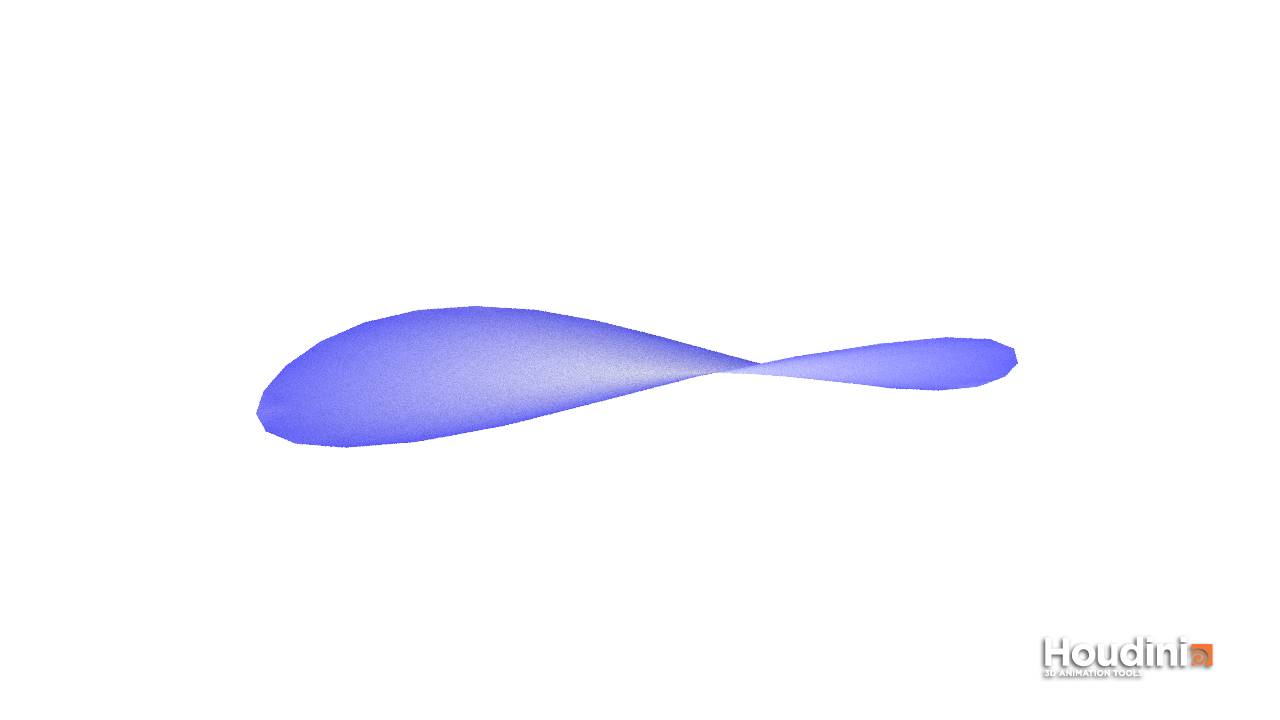
\includegraphics[width=\linewidth]{WetRimSim1.png} 
\caption{Caption1}
\label{fig:subim1}
\end{subfigure}%
\hfill
\begin{subfigure}{0.5\textwidth}
\centering
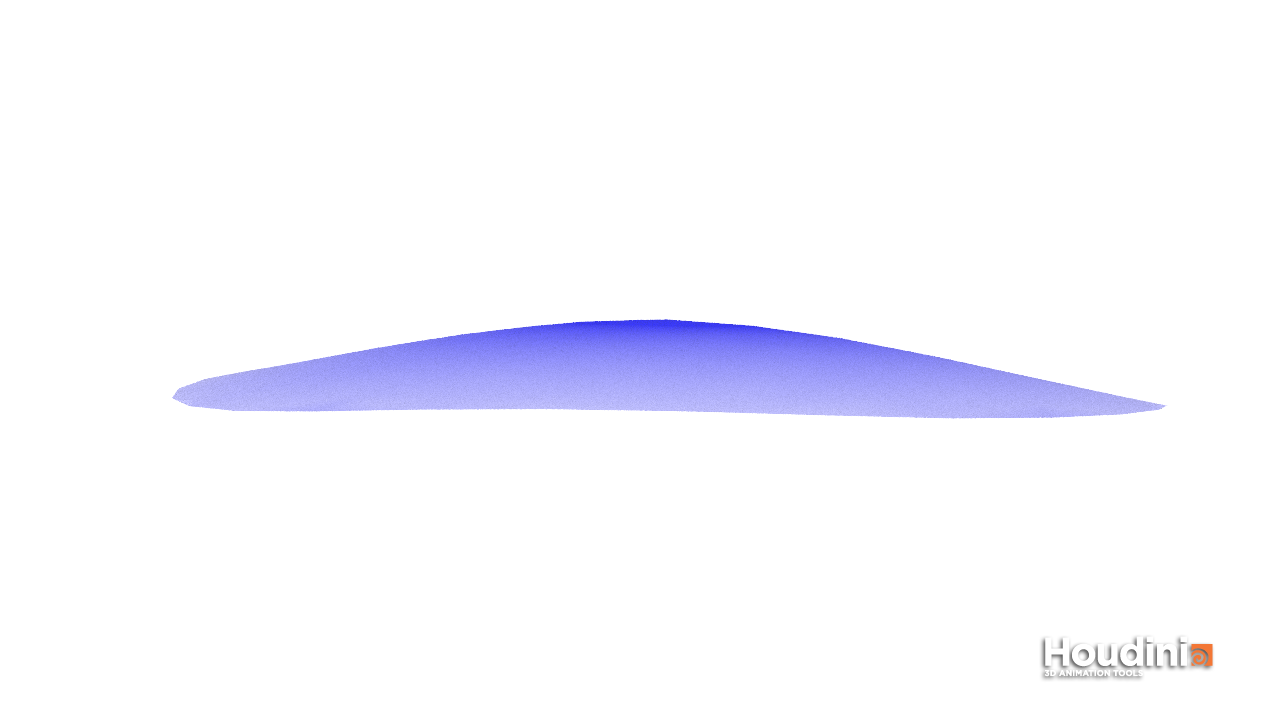
\includegraphics[width=\linewidth]{WetCenterSim2.png}
\caption{Caption 2}
\label{fig:WetDisc}
\end{subfigure}%

\end{figure}

\subsubsection{Machine Direction Experiment}
\begin{figure}[h]

\begin{subfigure}{0.45\textwidth}
\centering
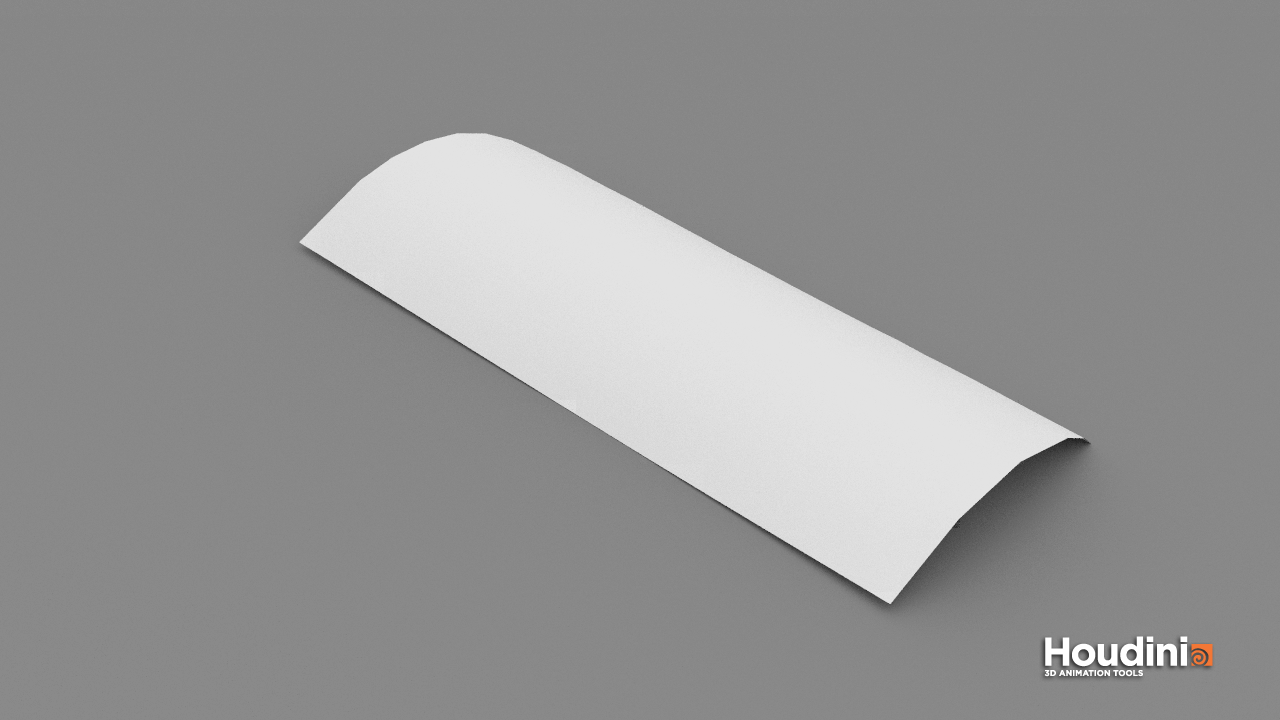
\includegraphics[width=\linewidth]{RechSim1.png} 
\caption{Caption1}
\label{fig:subim1}
\end{subfigure}%
\hfill
\begin{subfigure}{0.45\textwidth}
\centering
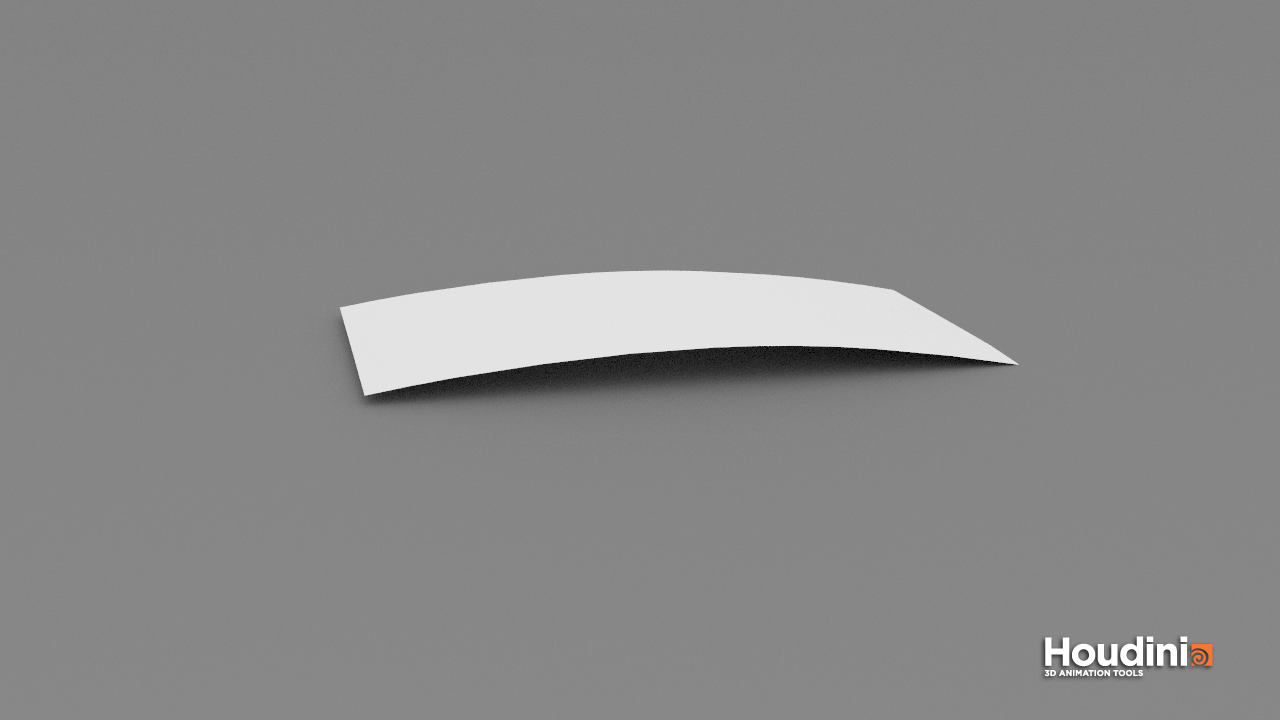
\includegraphics[width=\linewidth]{RecvSim1.png}
\caption{Caption 2}
\label{fig:Rec}
\end{subfigure}%

\end{figure}

\subsubsection{Dried Leaves}
\begin{figure}[h]
 
\begin{subfigure}{0.45\textwidth}
\centering
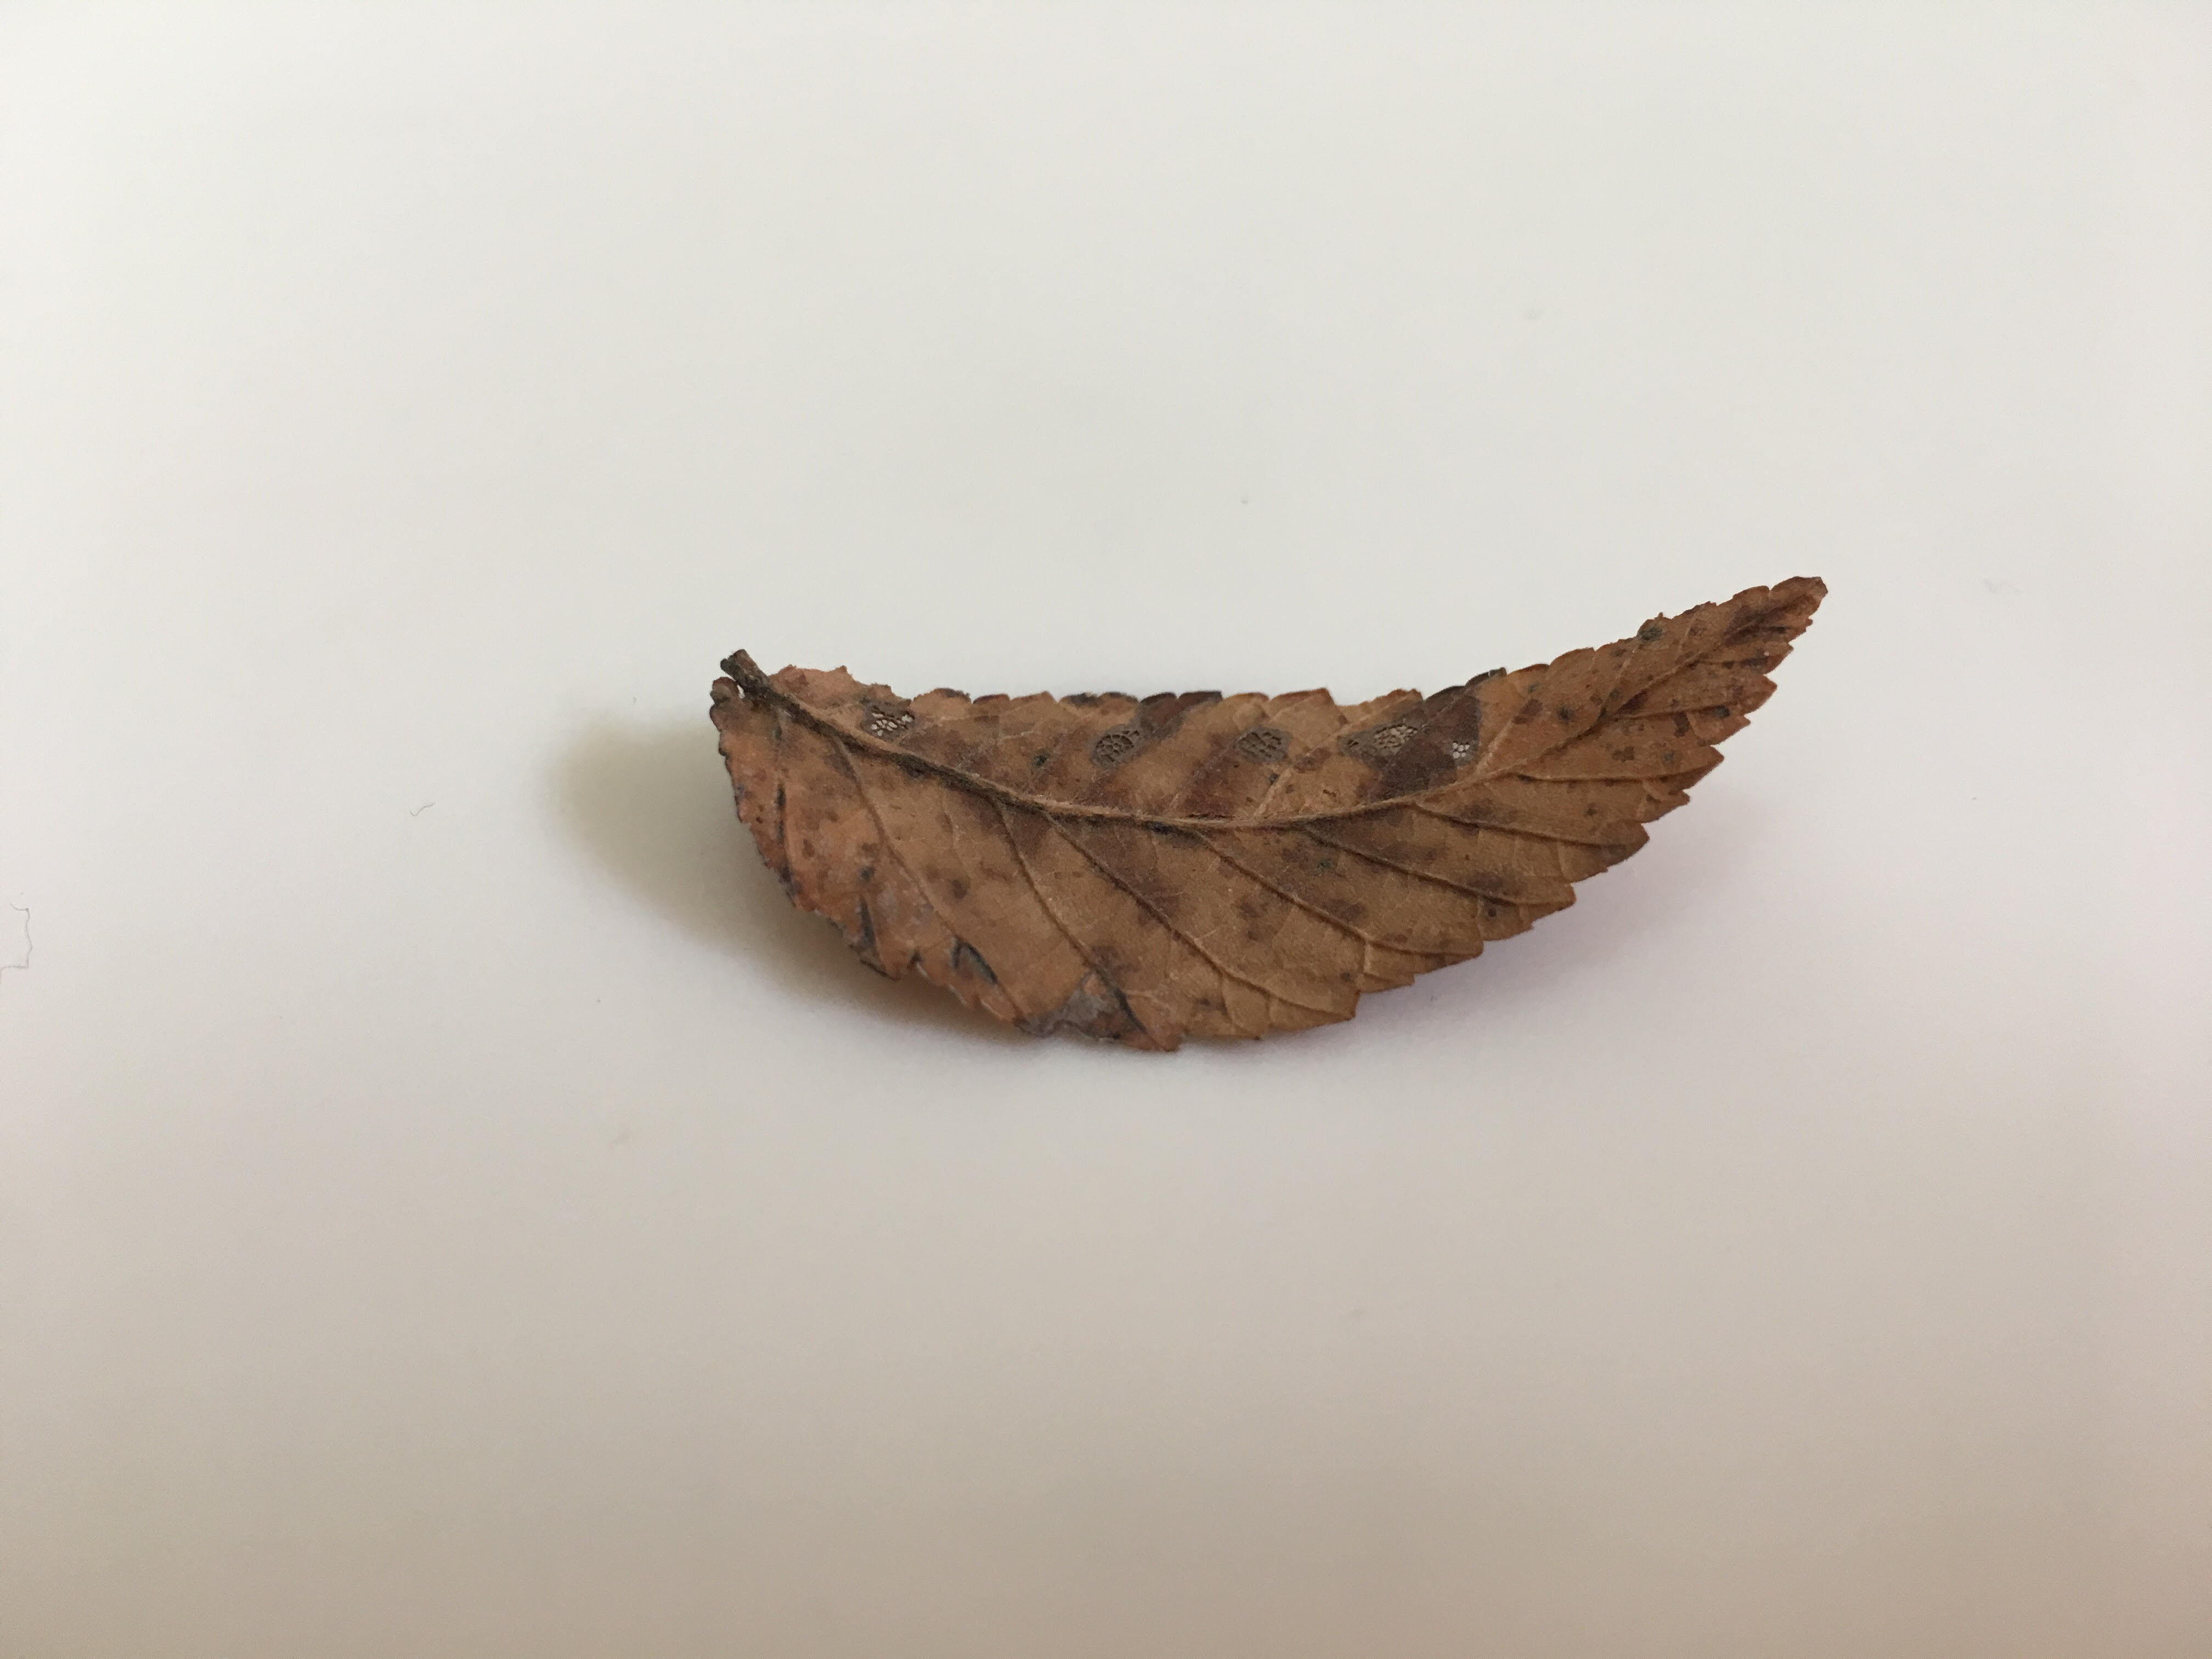
\includegraphics[width=0.45\linewidth]{actualLeafH2.jpg} 
\caption{Caption1}
\label{fig:subim1}
\end{subfigure}%
\hfill
\begin{subfigure}{0.45\textwidth}
\centering
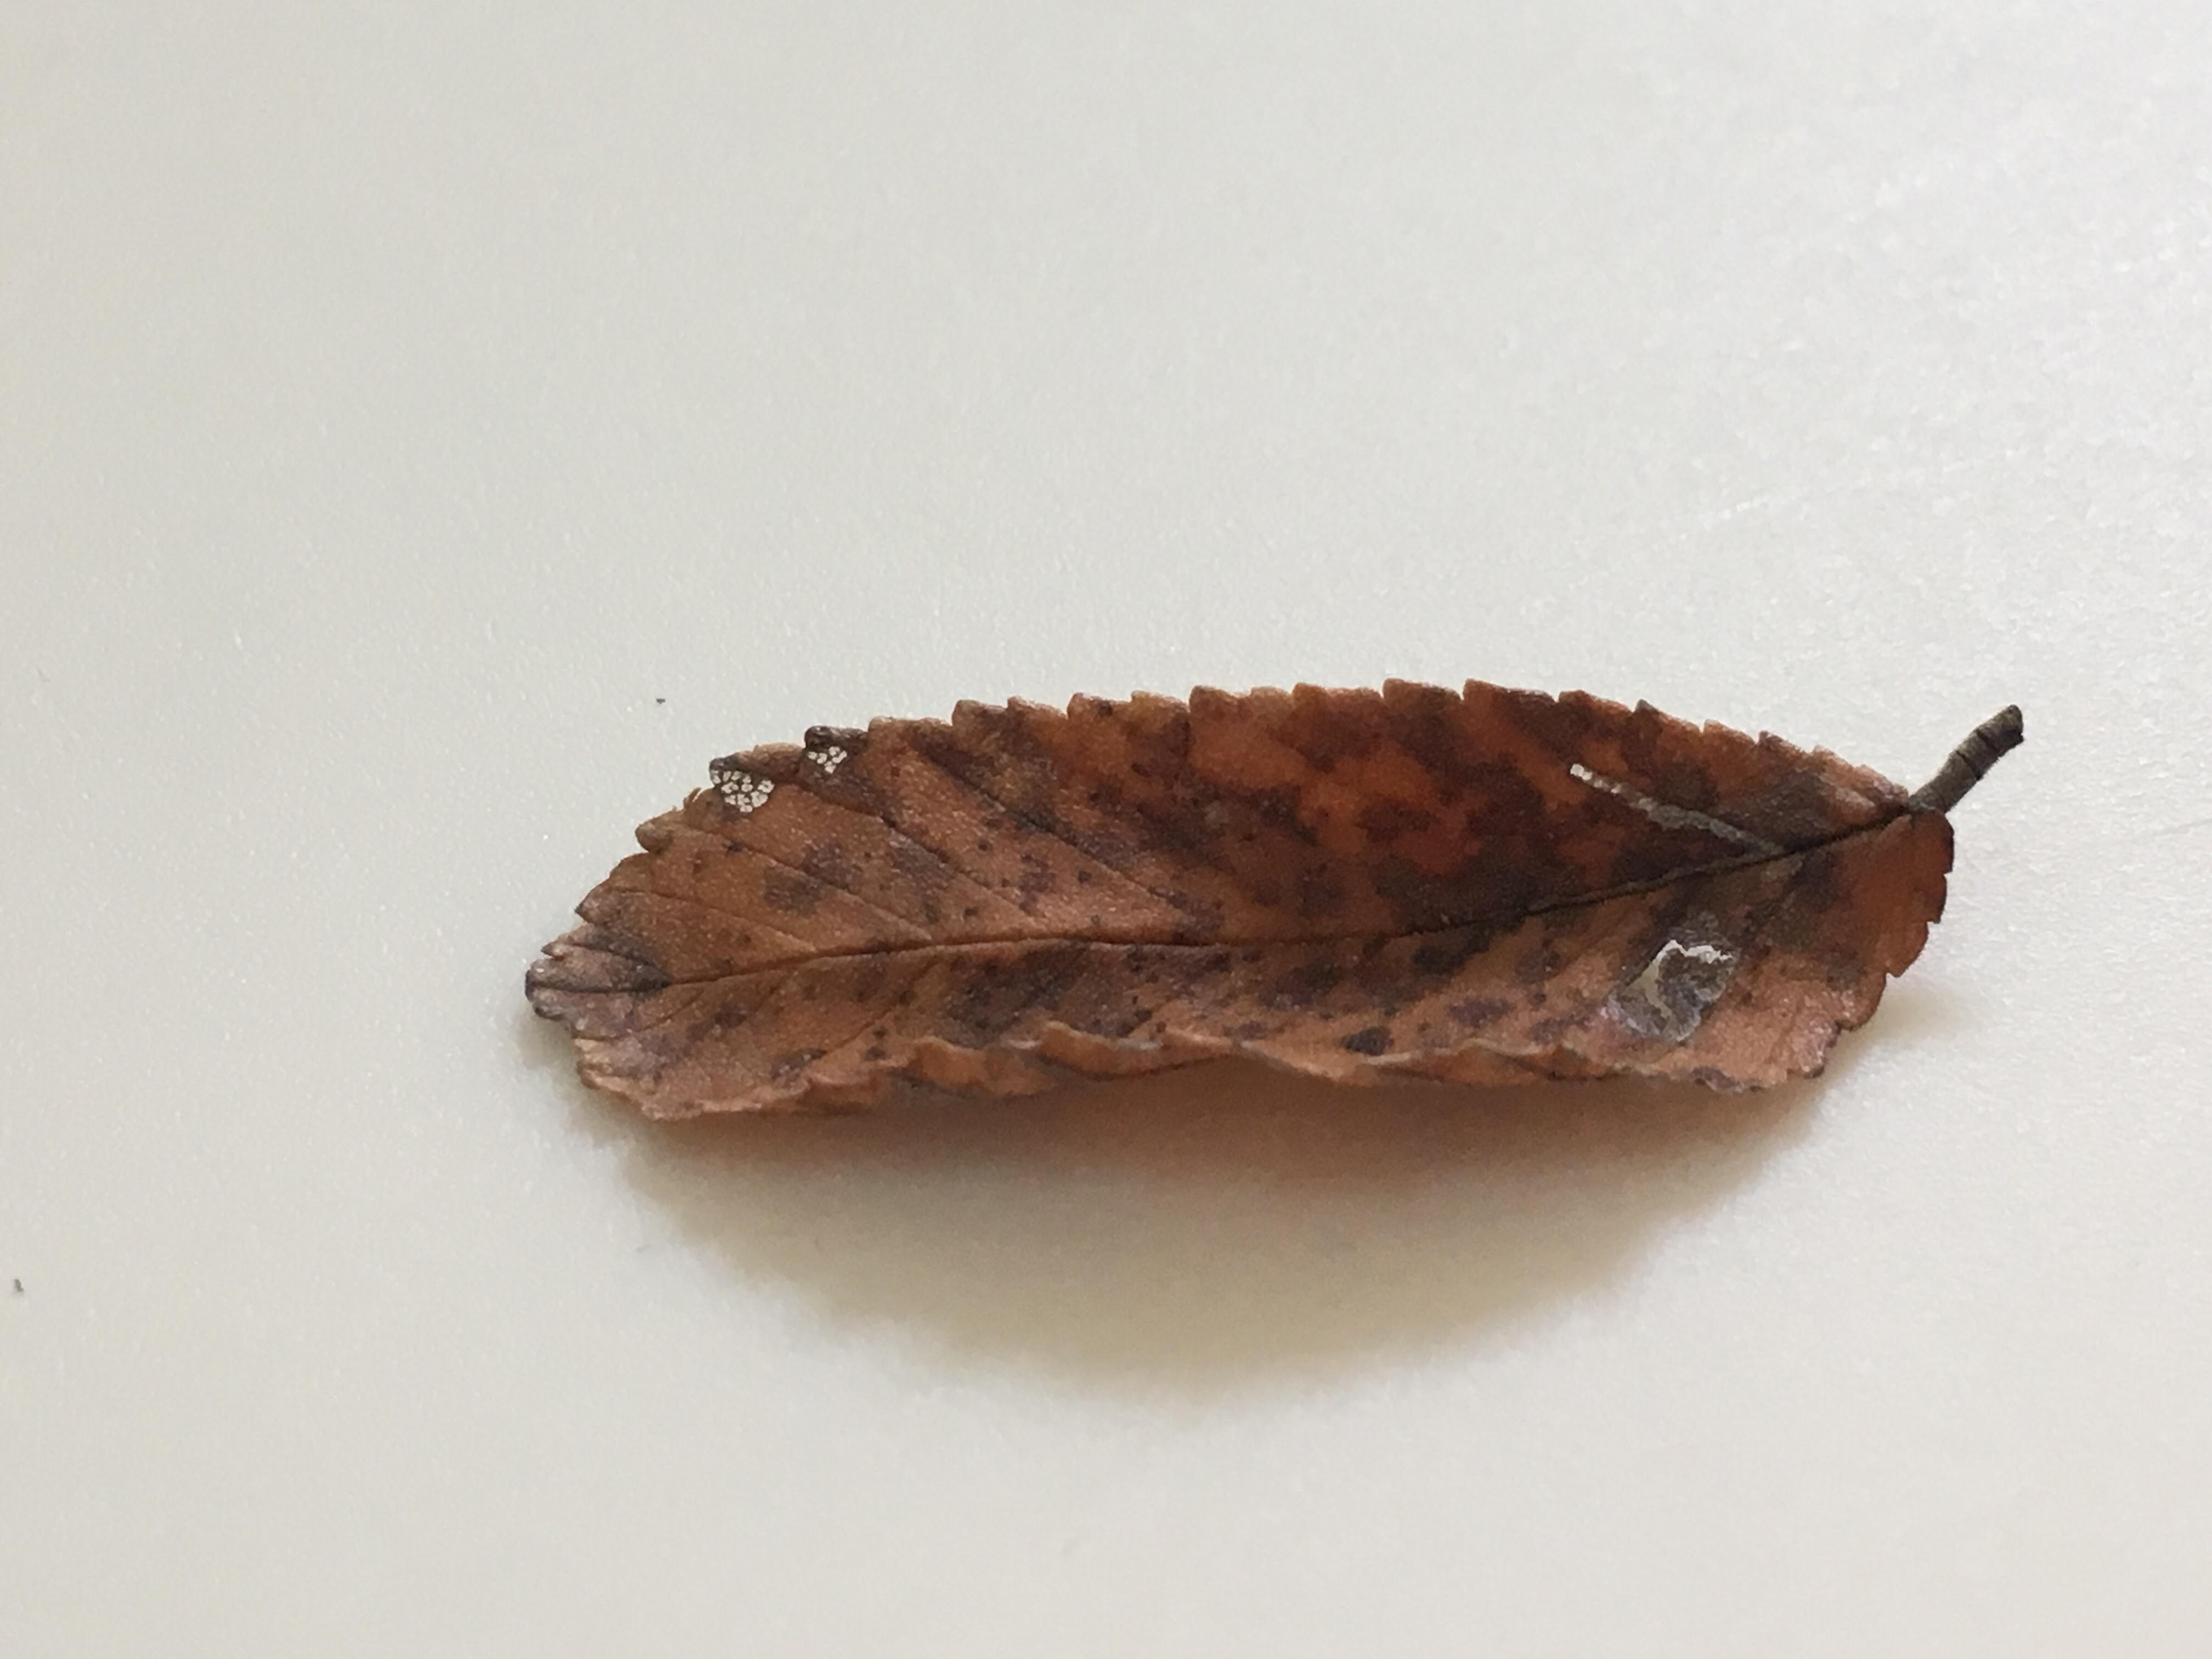
\includegraphics[width=0.45\linewidth]{actualLeafV.jpg}
\caption{Caption 2}
\label{fig:DriedLeaf}
\end{subfigure}%

\bigskip

\begin{subfigure}{0.45\textwidth}
\centering
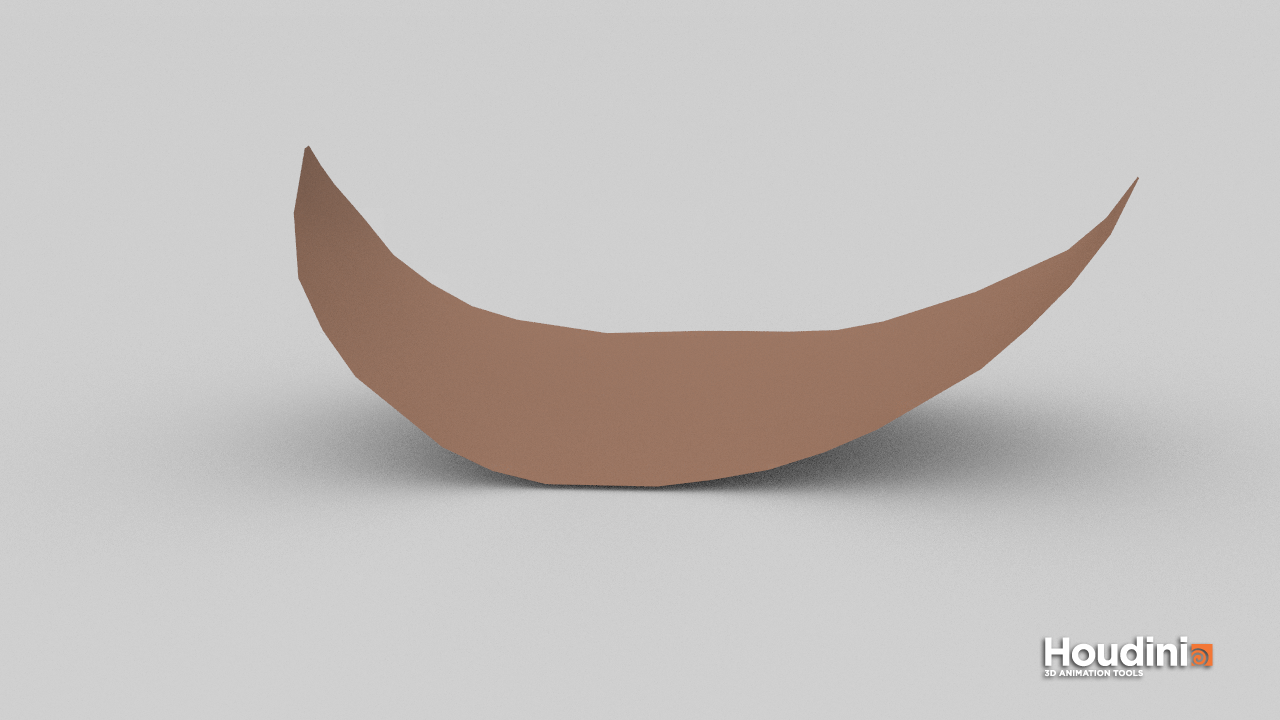
\includegraphics[width=0.45\linewidth]{LeafhSim1.png} 
\caption{Caption1}
\label{fig:subim3}
\end{subfigure}%
\hfill
\begin{subfigure}{0.45\textwidth}
\centering
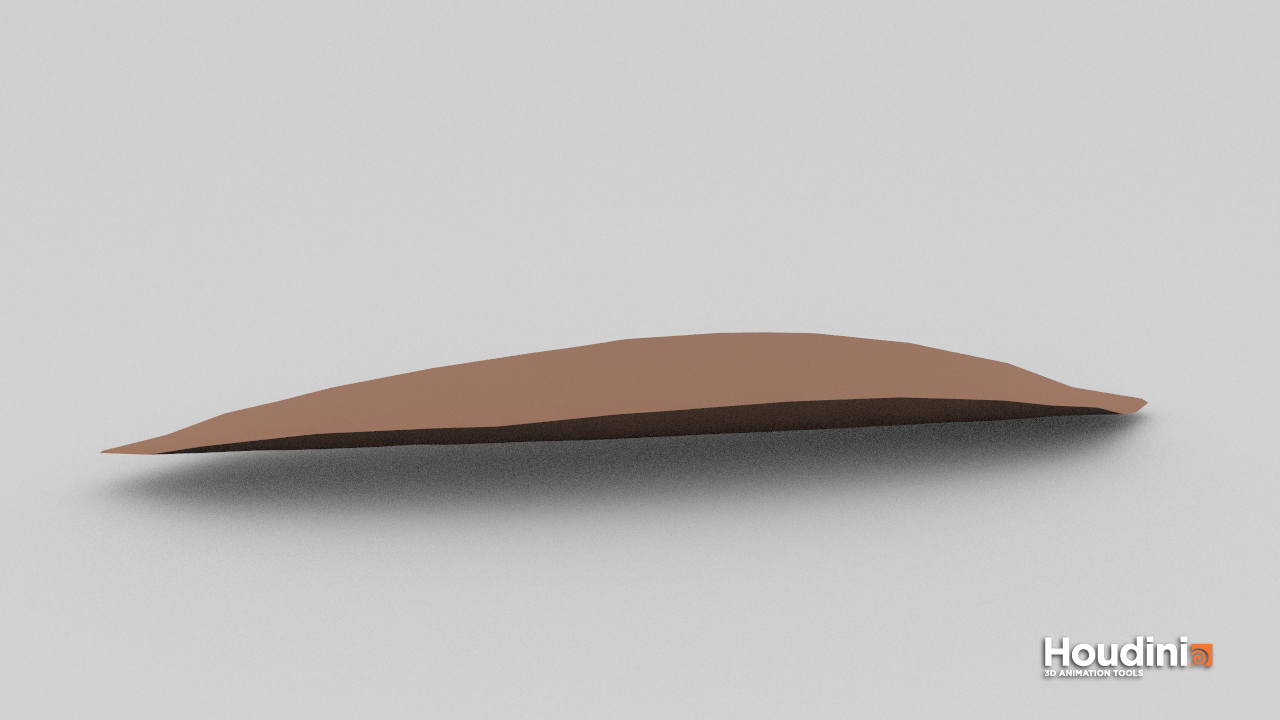
\includegraphics[width=0.45\linewidth]{LeafvSim1.png}
\caption{Caption 2}
\label{fig:subim4}
\end{subfigure}%
 
\caption{Simulation for Dried Leaves}
\label{fig:image2}
\end{figure}
\subsubsection{Wetting Paper Annulus}
\begin{figure}[h]
 
\begin{subfigure}{0.45\textwidth}
\centering
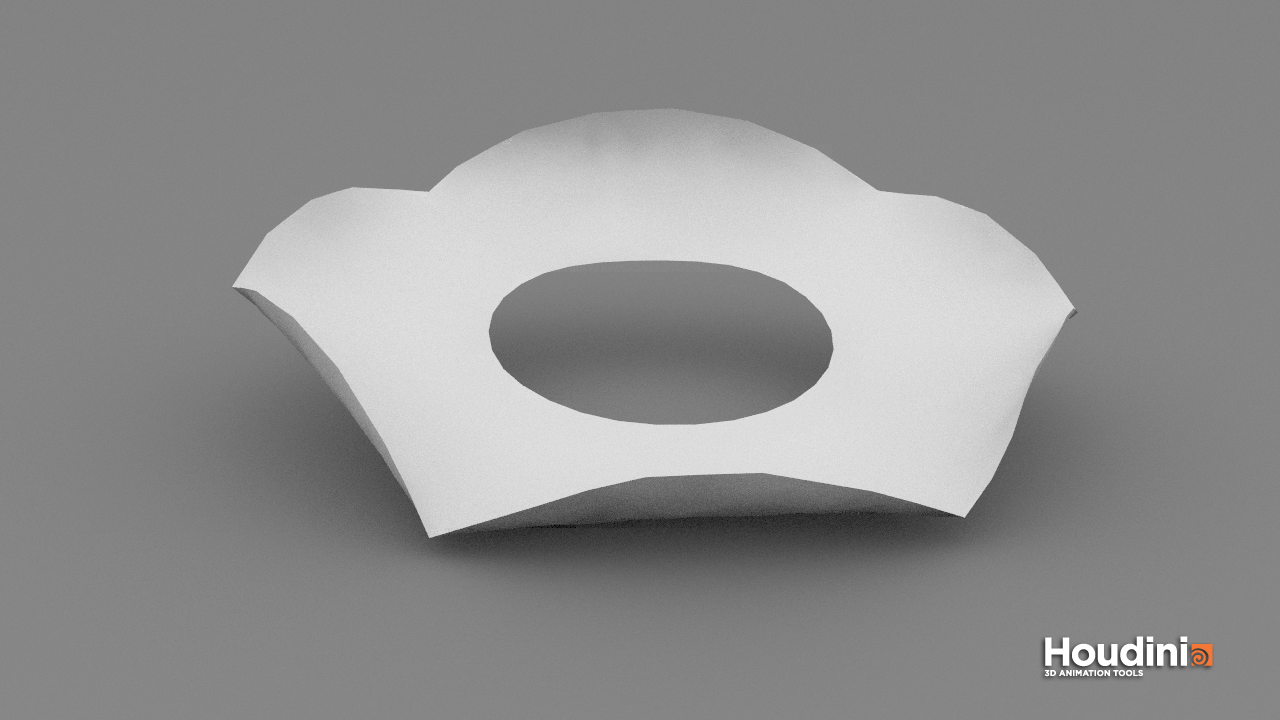
\includegraphics[width=0.45\linewidth]{AnnulusSim1.png} 
\caption{Caption1}
\label{fig:subim1}
\end{subfigure}%
\hfill
\begin{subfigure}{0.45\textwidth}
\centering
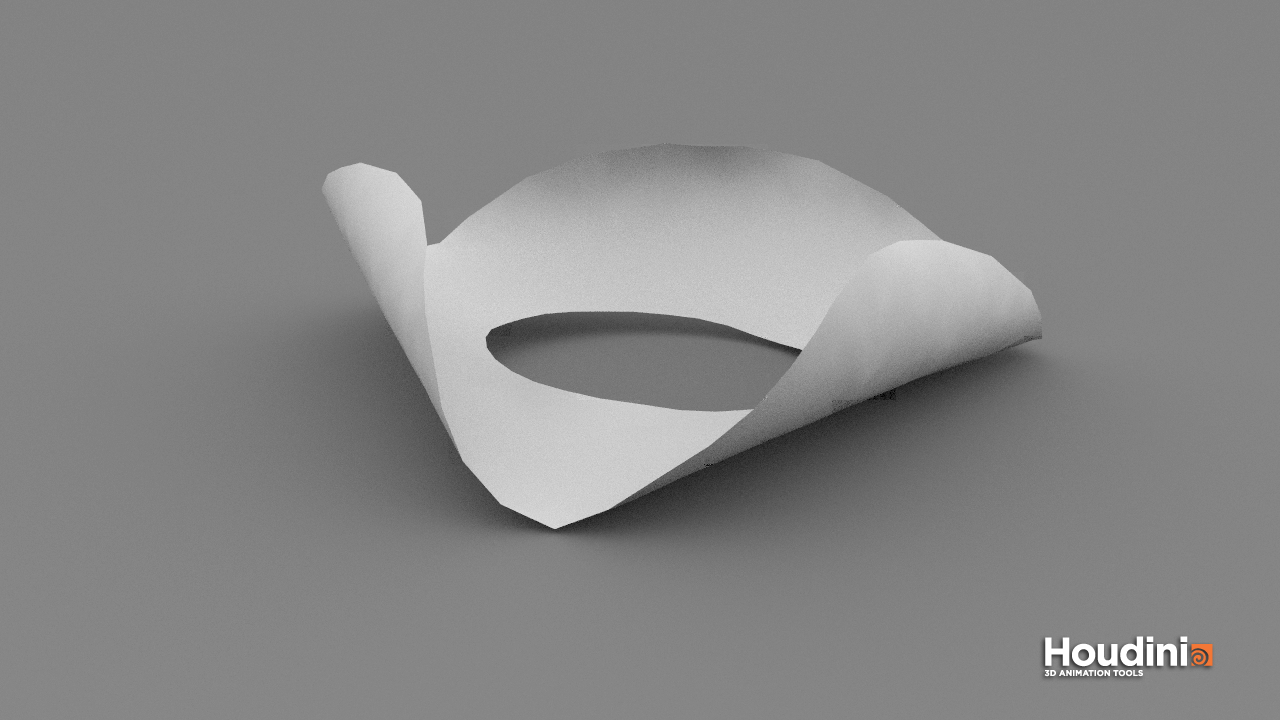
\includegraphics[width=0.45\linewidth]{AnnulusSim2.png}
\caption{Caption 2}
\label{fig:DriedLeaf}
\end{subfigure}%

\bigskip

\begin{subfigure}{0.45\textwidth}
\centering
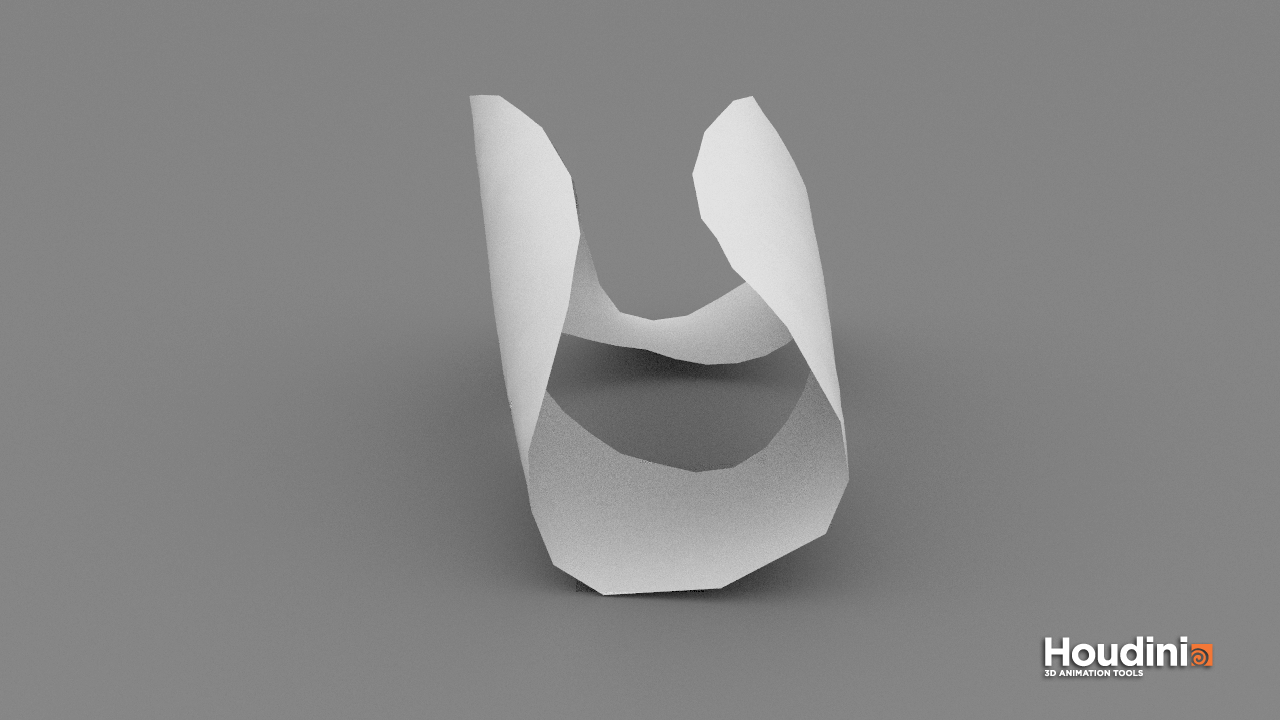
\includegraphics[width=0.45\linewidth]{AnnulusSim3.png} 
\caption{Caption1}
\label{fig:subim3}
\end{subfigure}%
 
\caption{Simulation for Wet Annulus}
\label{fig:image2}
\end{figure}

\subsubsection{Wetting Straw Wrapping Paper}
\subsubsection{Melting Spoon}
\subsubsection{Melting Torus}
\begin{figure}[h]
 
\begin{subfigure}{0.45\textwidth}
\centering
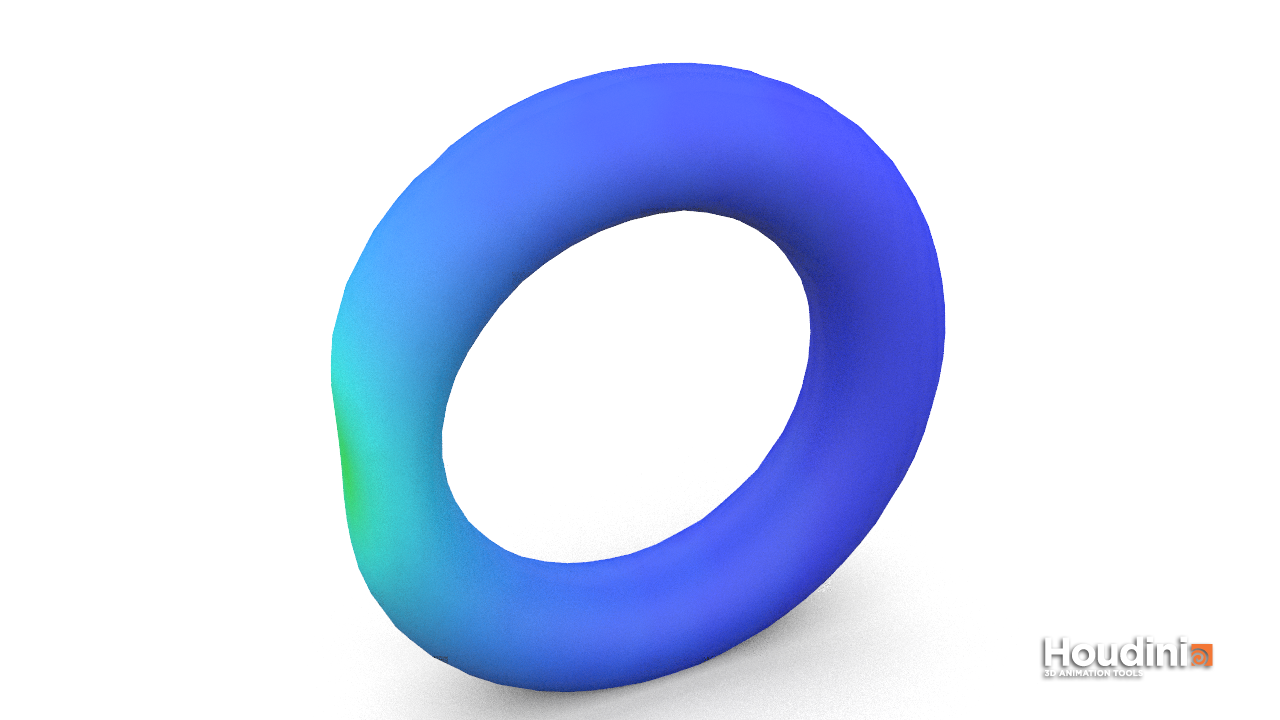
\includegraphics[width=0.45\linewidth]{TorusSim1.png} 
\caption{Caption1}
\label{fig:Torus1}
\end{subfigure}%
\hfill
\begin{subfigure}{0.45\textwidth}
\centering
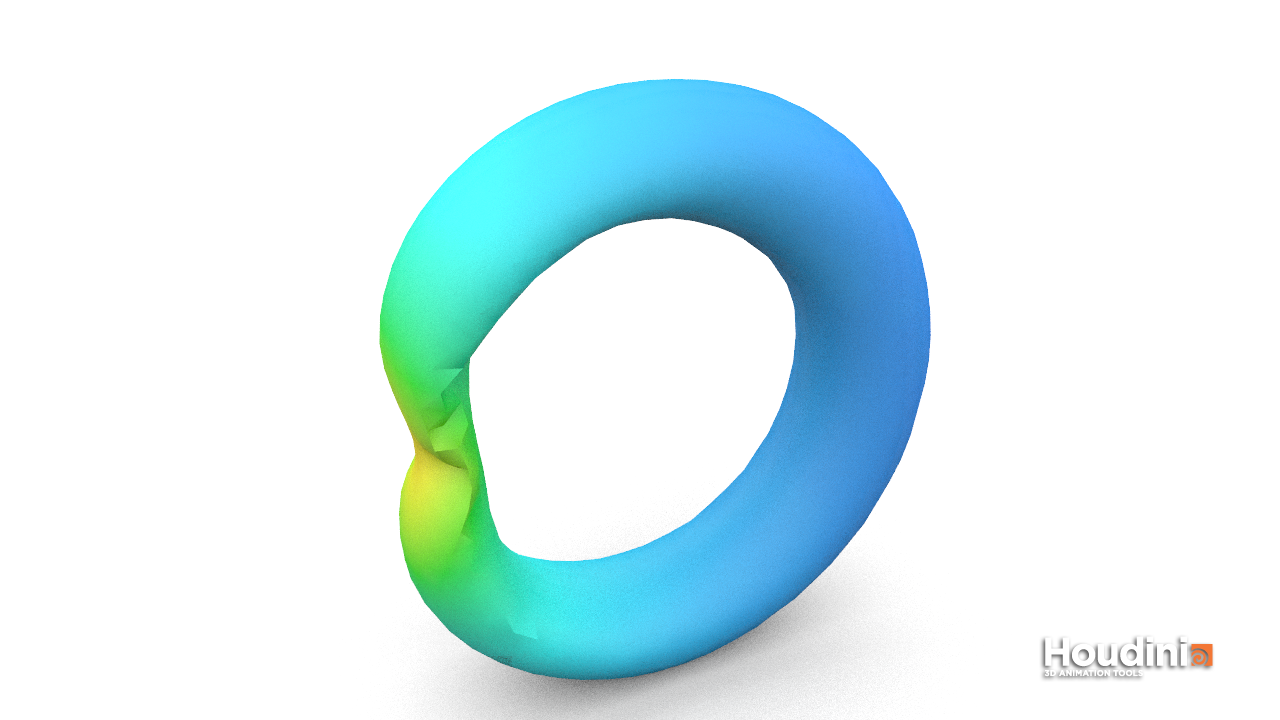
\includegraphics[width=0.45\linewidth]{TorusSim2.png}
\caption{Caption 2}
\label{fig:Torus2}
\end{subfigure}%

\bigskip

\begin{subfigure}{0.45\textwidth}
\centering
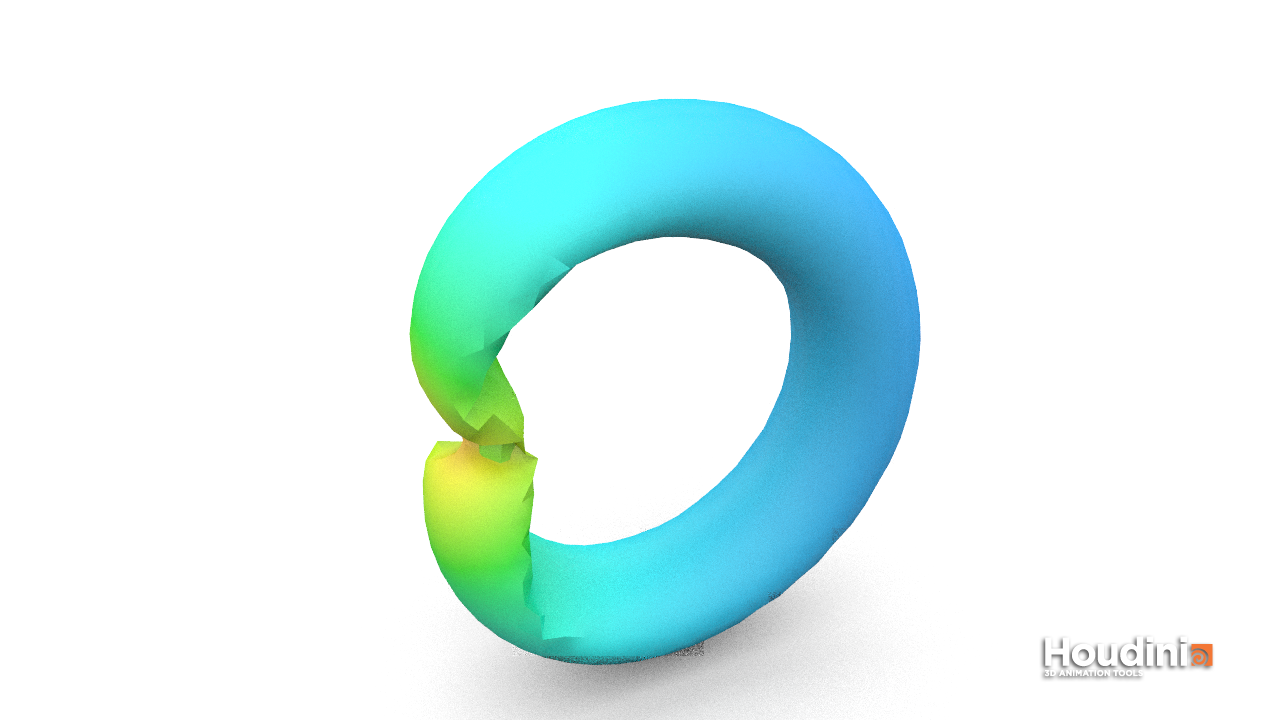
\includegraphics[width=0.45\linewidth]{TorusSim3.png} 
\caption{Caption1}
\label{fig:Torus3}
\end{subfigure}%
 
\caption{Simulation for Dried Torus}
\label{fig:Torus}
\end{figure}

\section{Conclusions and Future Work}

%Nullam vulputate enim ut tortor mollis pharetra. Cras pellentesque sem a accumsan malesuada. Donec at massa nisl. Sed malesuada felis id nisl maximus efficitur. In pretium metus non faucibus pulvinar. Sed pulvinar elit ultrices mauris vehicula, id ultricies purus finibus. Fusce tempus elit molestie, consequat ipsum eget, iaculis nibh. Cras tincidunt, orci in lacinia tempus, mauris leo finibus orci, vitae dignissim dui risus et odio. Sed commodo ultricies nulla, et varius velit aliquam quis. Sed efficitur, ex non facilisis dignissim, lacus orci accumsan massa, dictum facilisis arcu lacus ac leo. Sed quis tellus dictum massa egestas dapibus vel et justo. Nulla euismod lectus ut purus hendrerit porttitor. Suspendisse quis dui ligula. Proin non porta libero. Maecenas vel feugiat urna.
%
%\begin{acks}
%The authors would like to thank Dr. Yuhua Li for providing the MATLAB code of the \textit{BEPS} method.
%The authors would also like to thank the anonymous referees for their valuable comments and helpful suggestions. The work is supported by the \grantsponsor{GS501100001809}{National Natural Science Foundation of China}{https://doi.org/10.13039/501100001809} under Grant No.: ~\grantnum{GS501100001809}{61273304}
%21 and ~\grantnum[http://www.nnsf.cn/youngscientists]{GS501100001809}{Young Scientists' Support Program}.
%\end{acks}
